%! Suppress = MissingImport
%! Suppress = TooLargeSection
%! Suppress = SentenceEndWithCapital
%! Suppress = LineBreak
%! Suppress = MissingLabel
%! Suppress = Unicode

\documentclass[main.tex]{subfiles}

\begin{document}


    \section{Reprezentacja liczb całkowitych; arytmetyka.}

    \subsection{Kod znak-moduł prosty}
    \subsubsection{Reguły:}
    \begin{enumerate}
        \item Sygnalizacja znaku poprzez najwyższą pozycję
        rejestru (najczęściej pierwszą pozycję od lewej).
        \item Cyfra 0 na pozycji znaku oznacza dodatniość.
        \item Niezerowa cyfra na pozycji znaku oznacza ujemność.
        \item Cyfry określające wartość liczby (pozostałe cyfry) bez zmian (bez żadnego kodowania).
    \end{enumerate}
    \subsubsection{Przykłady:}
    \begin{itemize}
        \item Przykład w systemie dziesiętnym, q = 10,
        c = 5, u = 2, n = 8.\\
        $[+216.7]_{zmp} = 0|00216.70$\\
        $[-216.7]_{zmp} = 1|00216.70$
        \item Przykład w systemie binarnym, q = 2, c = 10,
        u = 5, n = 16.\\
        $[+1001100.101]_{zmp} = 0|0000100110.10100$\\
        $[-1001100.101]_{zmp} = 1|0000100110.10100$
    \end{itemize}
    \subsubsection{Arytmetyka}
    Kodowanie znak-moduł prosty przez swoją skomplikowaną
    i czasochłonną arytmetykę nie nadaje się do praktycznego
    stosowania (konieczność niestandardowego obsługiwania przepełnień)

    \subsection{Kod odwrotnościowy}
    \subsubsection{Reguły}
    \begin{itemize}
        \item Najbardziej znacząca cyfra (najczęściej lewa) jest cyfrą znaku.
        \item Zerowa cyfra znaku oznacza dodatniość.
        \item Najwyższa (ostatnia) cyfra znaku oznacza ujemność.
        \item Cyfry wartości liczby dodatniej pozostają bez zmian
        \item Cyfry wartości dla liczby ujemnej:
        \begin{itemize}
            \item W systemie dwójkowym są odwróceniem bitów.
            \item W systemie dziesiętnym są uzupełnieniem każdej cyfry
            do liczby 9.
            \item Ogólnie są uzupełnienie każdej cyfry do najwyższej cyfry
            systemu, czyli do wartości q-1.
        \end{itemize}
    \end{itemize}

    \subsubsection{Przykłady}
    \begin{itemize}
        \item System dziesiętny:
        q = 10, c = 7, u = 5
        \begin{align*}
        [-182073.6954]
            _{odw} = [-0|0182073.69540]_{odw} = 9|9917926.30459
        \end{align*}

        \item - System binarny:
        q = 2, c = 7, u = 5
        \begin{align*}
        [-101110.011]
            _{odw} = [-0|0101110.01100]_{odw} = 1|0010001.10011
        \end{align*}

    \end{itemize}

    \subsubsection{Arytmetyka}
    Algorytm sumowania:
    \begin{itemize}
        \item Dodaj kody, a w przypadku przepełnienia zwiększ wynik o najmniejszą możliwą liczbę dodatnią.
    \end{itemize}

    \subsubsection{Przykłady}
    \begin{itemize}
        \item W systemie dziesiętnym, q=10, c=7, u=5
        \begin{center}
            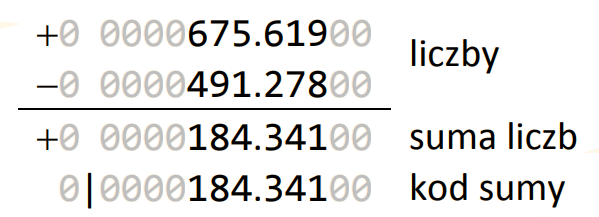
\includegraphics[scale=0.4]{number-repr/odw-add-dec.png}
        \end{center}
        \begin{center}
            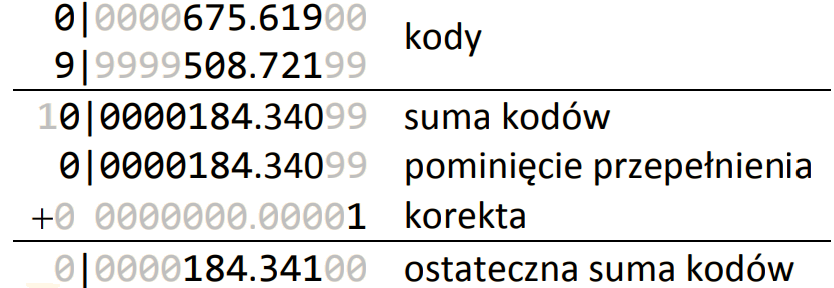
\includegraphics[scale=0.4]{number-repr/odw-add-dec-2.png}
        \end{center}


        \item w systemie binarnym, q=2, c=7, u=5
        \begin{center}
            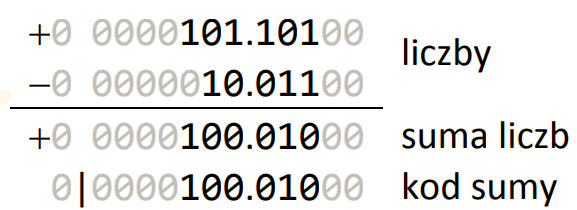
\includegraphics[scale=0.4]{number-repr/odw-add-bin.png}
        \end{center}
        \begin{center}
            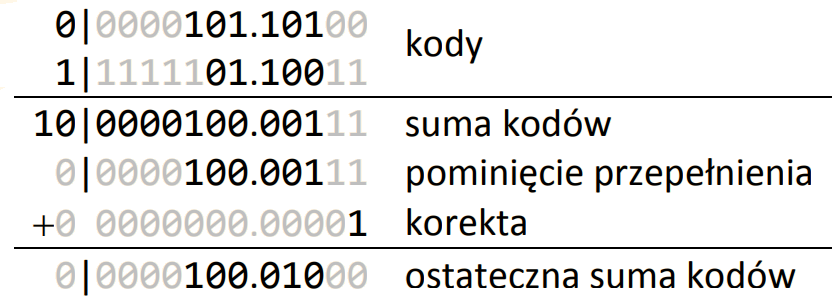
\includegraphics[scale=0.4]{number-repr/odw-add-bin-2.png}
        \end{center}

    \end{itemize}


    \subsection{Kod uzupełnieniowy}
    \subsubsection{Kodowanie}
    Kodowanie uzupełnieniowe liczby ujemnej polega na uzupełnieniu każdej cyfry do najwyższej
    cyfry systemu (odwróceniu bitów) i dodaniu do
    otrzymanej wartości liczby 1 na najmniej znaczącym miejscu.
    \subsubsection{Dekodowanie}
    Dekodowanie liczby ujemnej zakodowanej uzupełnieniowo polega na odjęciu od kodu liczby 1
    na najmniej znaczącym miejscu z uzupełnieniem
    w otrzymanym kodzie każdej cyfry do najwyższej
    cyfry systemu (odwróceniem bitów).

    \subsubsection{Przykłady kodowania}
    \begin{itemize}
        \item w systemie dziesiętnym (q = 10, c = 7, u = 5)
        \begin{center}
            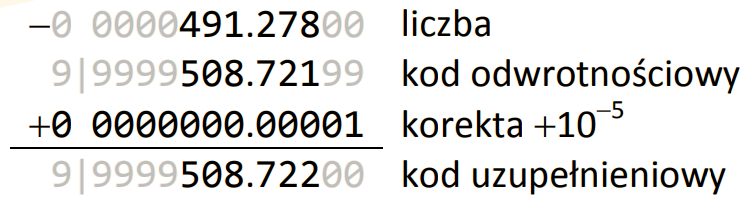
\includegraphics[scale=0.4]{number-repr/uzp-encode-dec.png}

        \end{center}
        \item w systemie binarnym q = 10, c = 7, u = 5.
        \begin{center}
            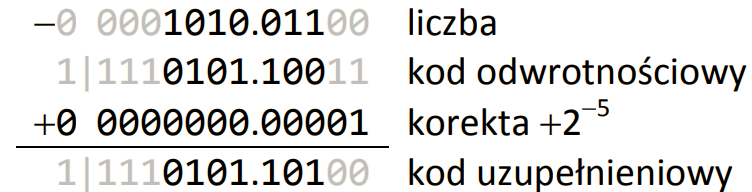
\includegraphics[scale=0.4]{number-repr/uzp-encode-bin.png}
        \end{center}

    \end{itemize}

    \subsubsection{Arytmetyka}
    Suma kodów uzupełnieniowych jest zawsze kodem uzupełnieniowym sumy.
    \begin{itemize}
        \item w systemie dziesiętnym  (q = 10, c = 7, u = 5)
        \begin{center}
            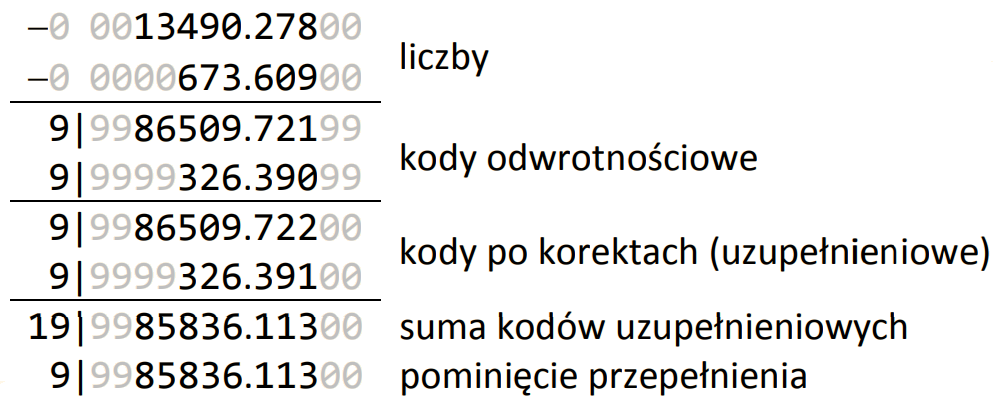
\includegraphics[scale=0.4]{number-repr/uzp-add-dec.png}
        \end{center}

        \item w systemie binarnym q = 10, c = 7, u = 5
        \begin{center}
            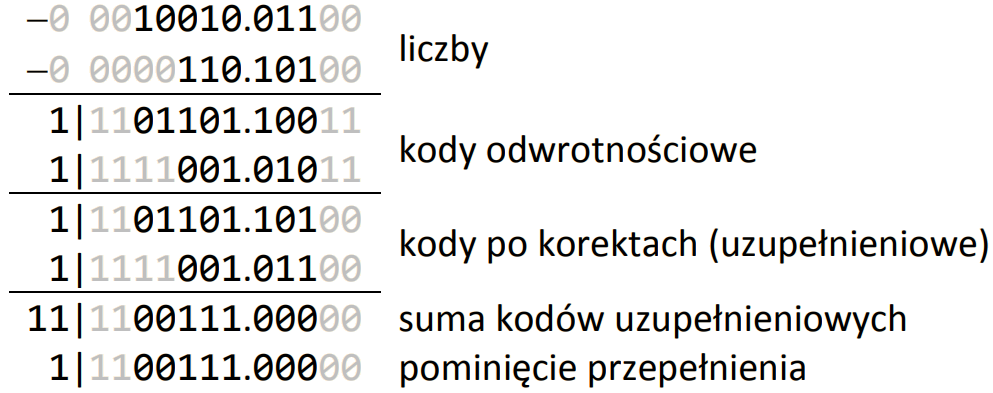
\includegraphics[scale=0.4]{number-repr/uzp-add-bin.png}
        \end{center}
    \end{itemize}

    \subsection{Kod nadmiarowy}
    \subsubsection{Kodowanie}
    \begin{enumerate}
        \item Kodowanie nadmiarowe liczby dodatniej polega na
        ustawieniu cyfry znaku na wartość jednostkową.
        \begin{center}
            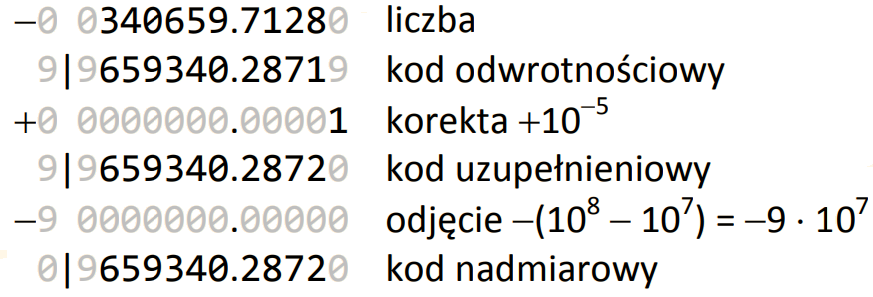
\includegraphics[scale=0.4]{number-repr/nad-encode-dec.png}
        \end{center}
        \item Kod nadmiarowy liczby ujemnej to kod uzupełnieniowy z odjęciem najwyższej cyfry systemu
        na pozycji znaku.
        \begin{center}
            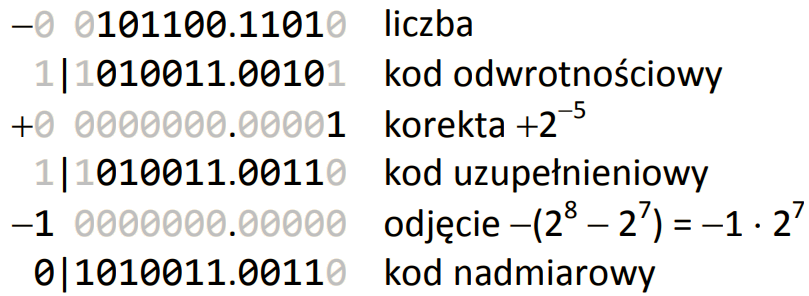
\includegraphics[scale=0.4]{number-repr/nad-encode-bin.png}
        \end{center}
    \end{enumerate}


    \subsubsection{Dekodowanie}
    \begin{itemize}
        \item Dekodowanie nadmiarowe kodu liczby dodatniej
        (rozpoznawanego po niezerowej cyfrze znaku) polega na wyzerowaniu cyfry znaku.
        \item Dekodowanie nadmiarowe kodu liczby ujemnej
        (rozpoznawanego po zerowej cyfrze znaku) wymaga
        ustawienia najwyższej cyfry systemu w miejscu znaku z następującym dekodowaniem uzupełnieniowym.
    \end{itemize}

    \subsubsection{Arytmetyka}
    Kod nadmiarowy sumy liczb to suma kodów nadmiarowych
    składników z odjętą wartością 1 na pozycji znaku.

    \begin{enumerate}
        \item w systemie dziesiętnym
        \begin{center}
            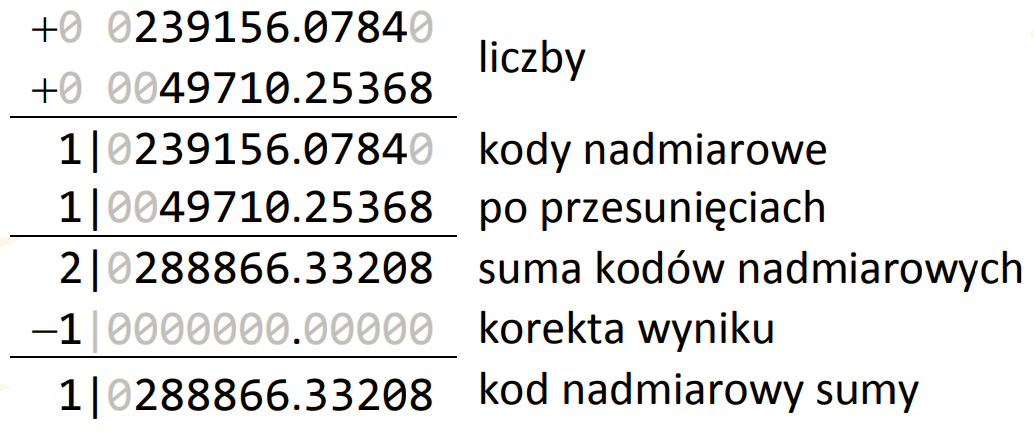
\includegraphics[scale=0.4]{number-repr/nad-add-dec.png}
        \end{center}
        \begin{center}
            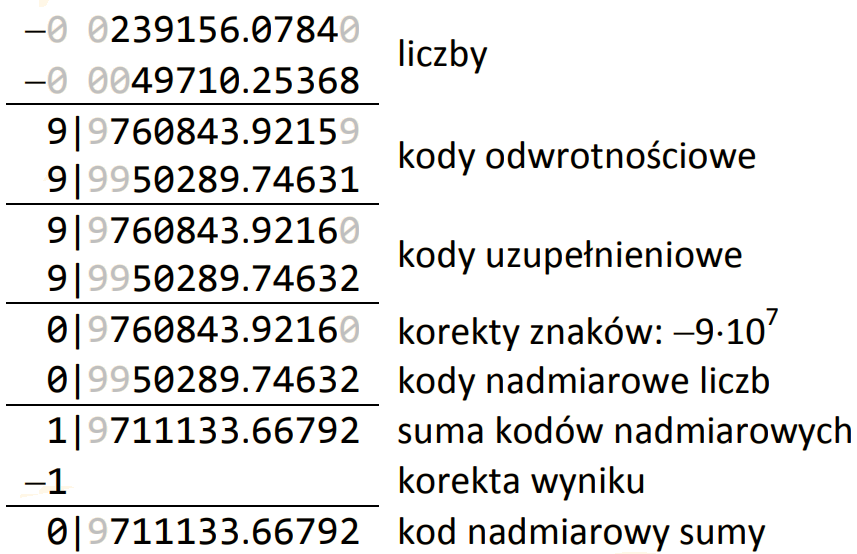
\includegraphics[scale=0.4]{number-repr/nad-add-dec-2.png}
        \end{center}

        \item w systemie binarnym
        \begin{center}
            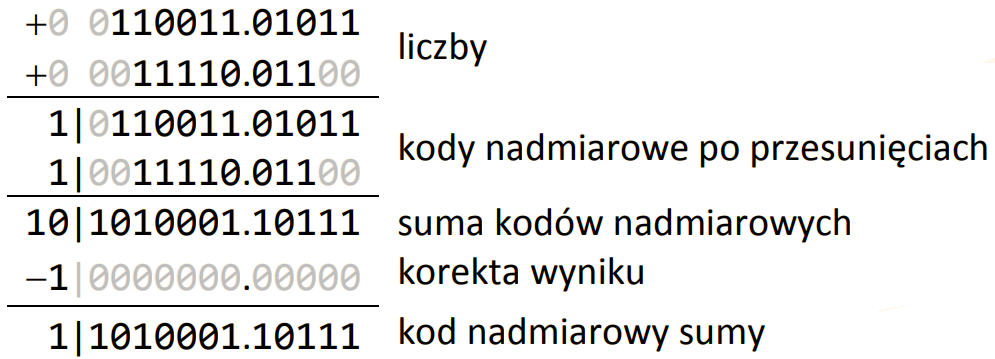
\includegraphics[scale=0.4]{number-repr/nad-add-bin.png}
        \end{center}
        \begin{center}
            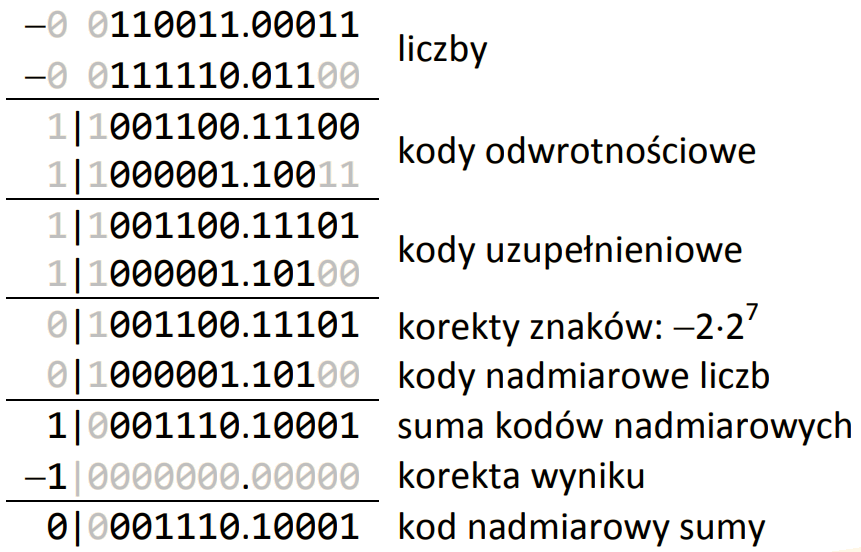
\includegraphics[scale=0.4]{number-repr/nad-add-bin-2.png}
        \end{center}
    \end{enumerate}






    \newpage

    \section{Reprezentacja liczb rzeczywistych; arytmetyka zmiennopozycyjna.}

    \subsection{Reprezentacja cecha-mantysa}
    Liczby postaci
    \begin{align*}
        m \times q^c
    \end{align*}
    gdzie m - mantysa, q - podstawa systemu liczbowego, c - cecha

    \begin{itemize}
        \item Mantysa - ciąg najbardziej znaczących cyfr liczby.
        \item Cecha - wykładnik potęgi podstawy systemu w iloczynie z mantysą równy reprezentowanej liczbie.
        \item W rejestrze komputera pamiętane są wyłącznie mantysa oraz cecha, zaś podstawa systemu jest ustalona, zatem nie musi być reprezentowana i nie jest konieczna do działań.
        \item Różnorodne sposoby zapamiętania w komputerze liczb w postaci cecha-mantysą noszą nazwę \textbf{kodowań zmiennopozycyjnych.}

    \end{itemize}

    \subsection{Kodowanie zmiennopozycyjne}
    \begin{itemize}
        \item Kodowanie zmiennopozycyjne jest powszechnie stosowanie w komputerach dla reprezentacji liczb rzeczywistych.
        \item W systemie dziesiętnym dla oddzielenia mantysy i cechy powszechne użycie litery E (lub e).
        Liczba 28.05
        \begin{center}
            \texttt{28.05e0 = 2805e-2 = +2805000e-5 =\\
            = 0.0002805e+5 = 2.805e1 = 0.2805e2}
        \end{center}

        \item W systemie binarnym dla oddzielenia mantysy i cechy powszechne użycie litery D (lub d).
        Liczba $(9.625)_{10} = (1001.101)_2$
        \begin{center}
            \texttt{0.00001001101d1000 = 1001101000d-110 =\\
            = 1.001101d11 = 0.1001101d100}
        \end{center}

        \item Różnorodność reprezentacji zmiennopozycyjnej wymusza konieczność ujednoznacznienia zwaną \textbf{normalizacją.}

    \end{itemize}

    \subsection{Normalizacja}

    \begin{table}
        \centering
        \begin{tabular}{l|l|l|l}
            & normalizacja
            całkowita & normalizacja
            do jedynki & normalizacja
            do ułamka  \\
            \hline
            28.05 & \texttt{2805e-2}                & \texttt{2.805e1}                  & \texttt{.2805e2}                  \\
            -35000000 & -\texttt{35e6}                & -\texttt{3.5e7}                   & -\texttt{.35e8}                   \\
            0.0000576 & \texttt{576e-6}                  & \texttt{5.76e-4}                  & \texttt{.576e-3}                  \\
            \hline
            $(1001.101)_2$    & \texttt{1001101d-11}             & \texttt{1.001101d11}              & \texttt{.1001101d100}             \\
            $(1010000)_2$     & \texttt{101d100}                 & \texttt{1.01d110}                 & \texttt{.101d111}                 \\
            $(-0.00001011)_2$ & -\texttt{1011d1001}              & -\texttt{1.011d111}               & -\texttt{.1011d1000}
        \end{tabular}
    \end{table}

    \subsection{Algorytmy kodowania i dekodowania}
    Przyjmujemy oznaczenia:
    \begin{itemize}
        \item $w_m$ - liczba cyfr reprezentacji mantysy (bez cyfry znaku)
        \item $w_c$ - liczba cyfr reprezentacji cechy (bez cyfry znaku)
        \item n - liczba cyfr rejestru
    \end{itemize}
    Zatem:
    \begin{align*}
        n = 1 + w_m + 1 + w_c
    \end{align*}

    \subsubsection{Algorytm kodowania}

    Algorytm kodowania zmiennopozycyjnego obejmuje poniższe kroki:
    \begin{enumerate}
        \item Przedstaw liczbę w systemie o podstawie q.
        \item Zaokrąglij wartość liczby do $w_m$ cyfr.
        \item Zaokrąglony wynik sprowadź do znormalizowanej postaci
        potęgowej $m\cdot q^c$
        \item Jeżeli cecha jest zbyt duża (zbyt dodatnia) by zmieścić się
        w przewidzianym zakresie $w_c$ to zasygnalizuj błąd przepełnienia i zakończ.
        \item Jeżeli cecha jest zbyt mała (zbyt ujemna) by zmieścić się
        w zakresie $w_c$ to zakoduj zerową mantysę oraz zerową wartość cechy i zakończ.
        \item Zakoduj stałopozycyjnie mantysę na $w_m + 1$ pozycjach.
        \item Zakoduj stałopozycyjnie cechę na $w_c + 1$ pozycjach.
    \end{enumerate}

    Przykłady dziesiętne:

    \begin{center}
        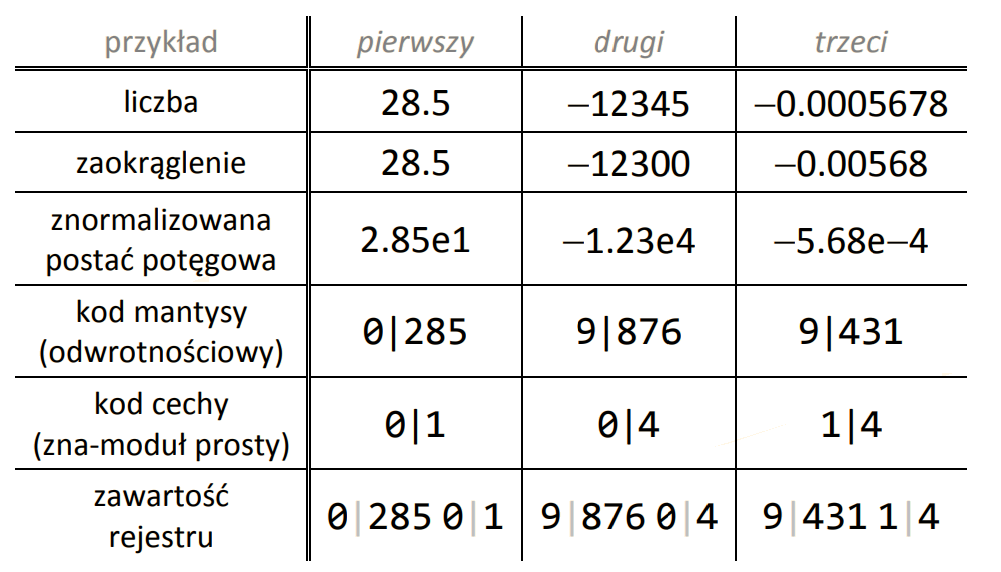
\includegraphics[scale=0.4]{number-repr/fl-pt-encode-dec.png}
    \end{center}

    Przykłady binarne:

    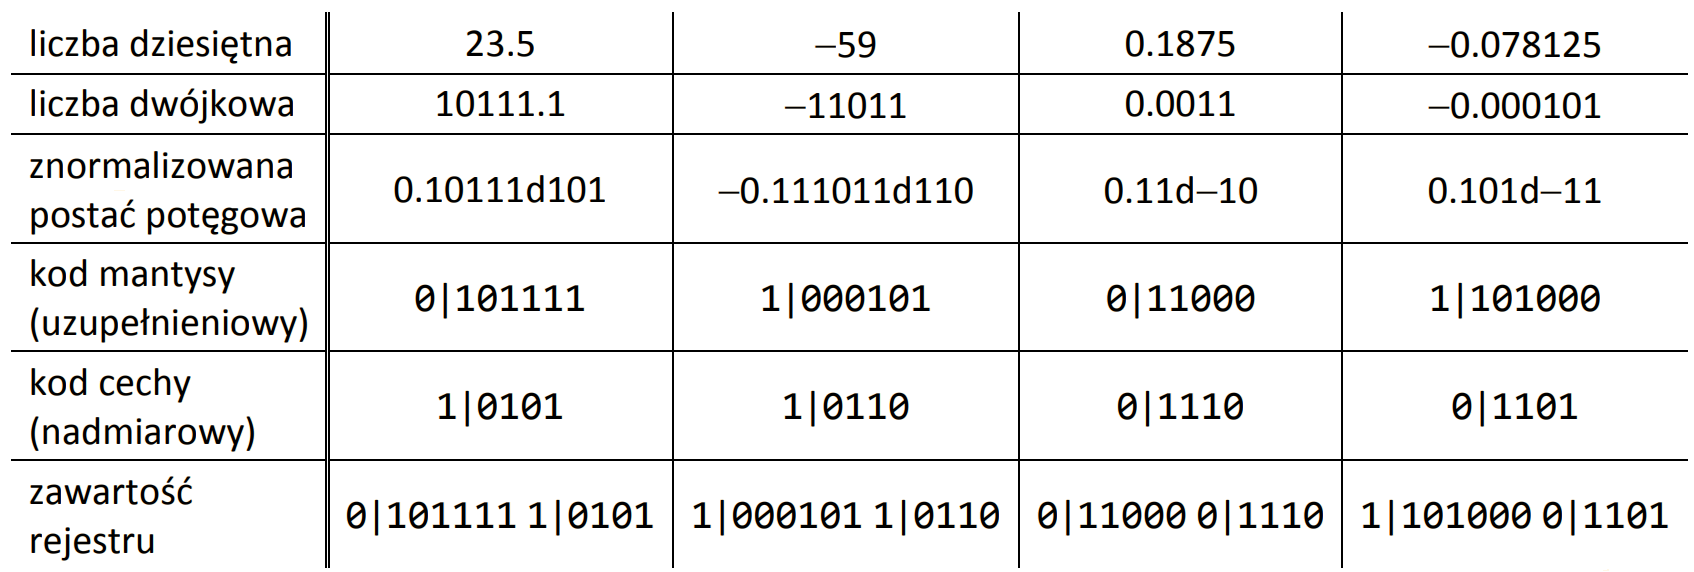
\includegraphics[width=\linewidth]{number-repr/fl-pt-encode-bin.png}

    \subsubsection{Algorytm dekodowania}

    System dziesiętny:
    \begin{enumerate}
        \item Dekoduj mantysę i cechę.
        \item Opcjonalnie eliminuj postać potęgową.
    \end{enumerate}

    System binarny:
    \begin{enumerate}
        \item Dekoduj mantysę i cechę.
        \item Sprowadź cechę do postaci dziesiętnej.
        \item Zdenormalizuj mantysę.
        \item Zapisz mantysę w postaci dziesiętnej.
    \end{enumerate}

    Przykłady binarne:

    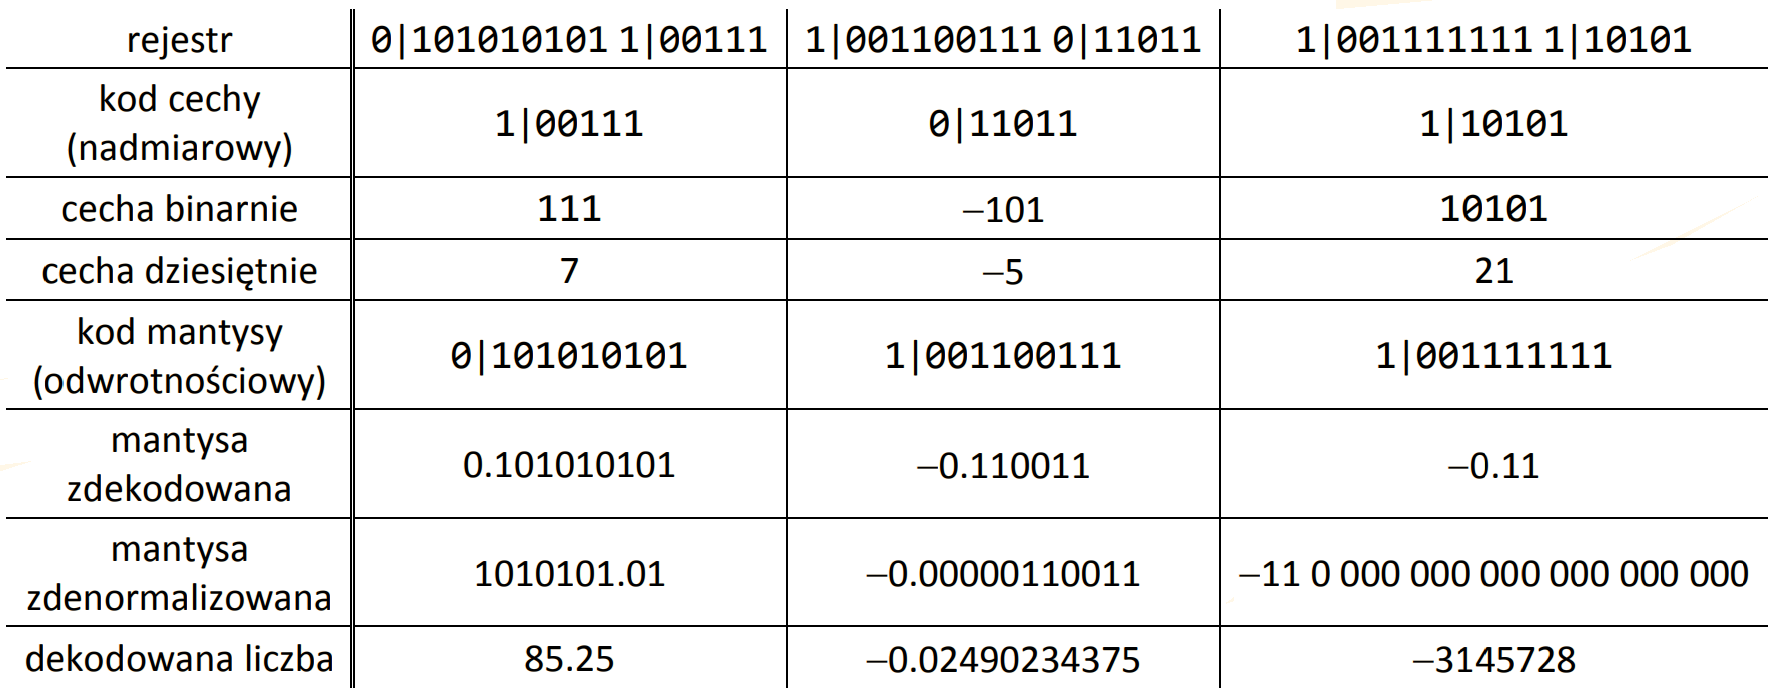
\includegraphics[width=\linewidth]{number-repr/fl-pt-decode-bin.png}

    \subsection{Arytmetyka}
    \begin{itemize}
        \item Brak ogólnego algorytmu działania na kodach
        zmiennopozycyjnych.
        \item Jedyna możliwa droga obejmuje oczywiste
        kroki:
        \begin{enumerate}
            \item Dekodowanie argumentów.
            \item Wykonanie działania.
            \item Zakodowanie wyniku.
        \end{enumerate}
    \end{itemize}

    \subsubsection{Dodawanie kodów zmiennopozycyjnych}
    Algorytm obejmuje kroki:
    \begin{enumerate}
        \item Zmodyfikuj mantysy dla zrównania cech (z możliwością
        denormalizacji).
        \item Wyznacz mantysę sumy w postaci sumy mantys (możliwe wobec równych cech).
        \item Zaokrąglij sumę mantys do liczby cyfr rejestru.
        \item Znormalizuj wynik sumy (skoryguj cechę wyniku).
    \end{enumerate}
    Przykład:\\
    \begin{center}
        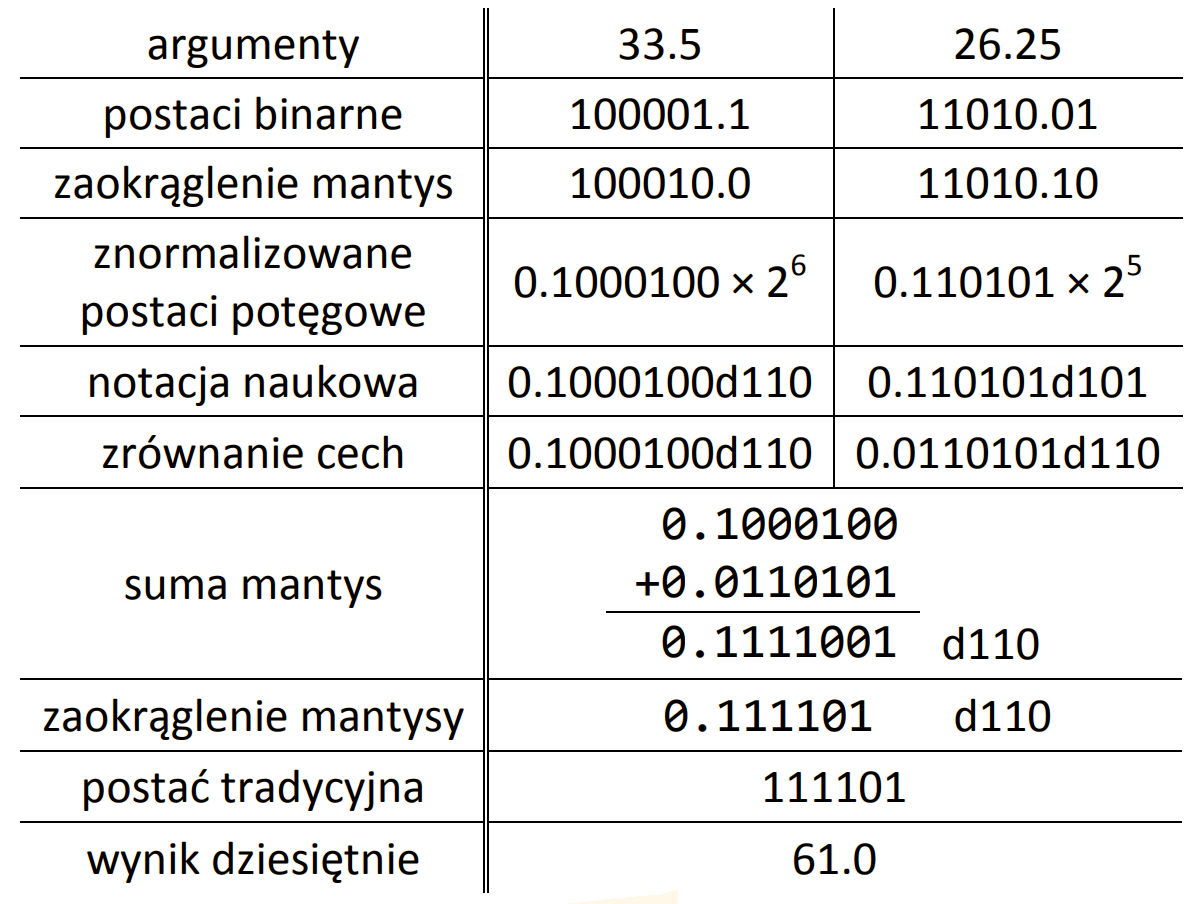
\includegraphics[scale=0.3]{number-repr/fl-pt-add.png}
    \end{center}

    \subsubsection{Mnożenie kodów zmiennopozycyjnych}
    Algorytm może obejmować kroki:
    \begin{enumerate}
        \item Mantysa iloczynu to iloczyn mantys, dlatego
        pomnóż mantysy.
        \item Cecha iloczynu to suma cech, zatem dodaj
        cechy.
        \item Zaokrąglij mantysę wyniku, iloczynu mantys.
        \item Znormalizuj mantysę modyfikując cechę.
    \end{enumerate}
    Przykład:\\
    \begin{center}
        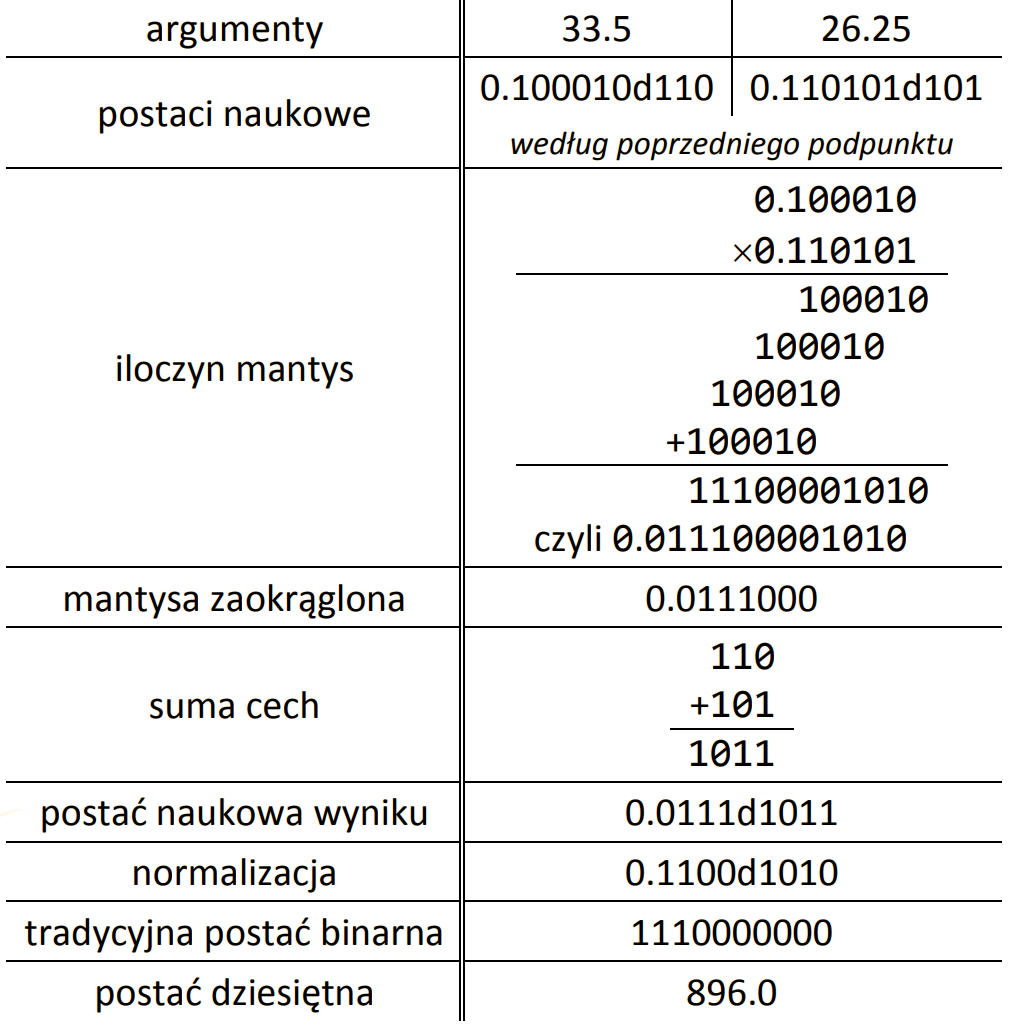
\includegraphics[scale=0.4]{number-repr/fl-pt-mult.png}
    \end{center}

    \newpage

    \section{Różnice w wywołaniu funkcji statycznych, niestatycznych i wirtualnych w C++.}

    \subsection{Funkcje statyczne.}
    \begin{itemize}
        \item \textbf{Globalne funkcje statyczne} to funkcje o zakresie widoczności ograniczonym do pliku źródłowego, który je
        zawiera (a dokładniej do ich \textit{jednostce translacji}, czyli pliku który jest kompilowany - zatem pliku
        źródłowego wraz z dołączonymi includami).
        \item \textbf{Metody statyczne klas} to metody których wywołanie jest niezależne od instancjonowania klasy -
        wszystkie instancje klasy współdzielą kopię statycznych metod i pól. Instancja klasy nie jest nam potrzebna
        do wywołania statycznej metody (aczkolwiek można jej użyć).
    \end{itemize}

    \begin{minted}{cpp}
        #include <iostream>
        using namespace std;

        // statyczna funkcja globalna dostępna tylko z naszego pliku
        static void sayHello(){
        cout << "hello" << endl;
        }

        class ExampleClass {
        public:
        static void sayBye(){
        cout << "bye" << endl;
        }
        };

        int main(){
        sayHello();

        ExampleClass::sayBye(); // wywołanie bez instancjonowania klasy

        ExampleClass e();
        e.sayBye(); // wywołanie dla instancji klasy
        }
    \end{minted}

    \subsection{Funkcje niestatyczne.}
    \begin{itemize}
        \item \textbf{Niestatyczne funkcje globalne} są dostępne ze wszystkich plików, które includują zawierające
        je plik źródłowy - trzeba zatem uważać na konflikty nazw.
        \item \textbf{Niestatyczne metody klas} wymagają do wywołania instancji klasy - mogą zachowywać się różnie
        dla różnych instancji; mogą być oznaczone \texttt{final} i \texttt{override}.
    \end{itemize}

    \begin{minted}{cpp}
        #include <iostream>
        using namespace std;

        // niestatyczna funkcja globalna dostępna dla wszystkich plików
        void sayHello(){
        cout << "hello" << endl;
        }

        class ExampleClass {
        public:
        void sayBye(){
        cout << "bye" << endl;
        }
        };

        int main(){
        sayHello();

        // ExampleClass::sayBye() - wywołanie niepoprawne

        ExampleClass e();
        e.sayBye(); // wywołanie dla instancji klasy
        }
    \end{minted}

    \subsection{Funkcje wirtualne.}
    \begin{itemize}
        \item \textbf{Wirtualne metody klas} są przydatne w polimorfizmie.
        \item W przypadku zwykłej metody, wywołanie jej dla wskaźnika typu klasy podstawowej zawsze wywoła instancję
        z klasy podstawowej, nawet jeżeli wskaźnik będzie tak naprawdę wskazywał na klasę pochodną.
        \item Słowo kluczowe \texttt{virtual} wymusza dedukcję której metody użyć na podstawie zawartości wskaźnika,
        a nie jego typu. Dedukcja następuje w czasie wykonania programu.
    \end{itemize}

    Bez \texttt{virtual}:
    \begin{minted}{cpp}
        #include <iostream>
        using namespace std;

        struct Base {
        void f() {
        cout << "base" << endl;
        }
        };

        struct Derived : Base {
        void f() {
        cout << "derived" << endl;
        }
        };

        int main(){
        Base b;
        Derived d;

        // call through reference
        Base& br = b; // the type of br is Base&
        Base& dr = d; // the type of dr is Base& as well
        br.f(); // "base"
        dr.f(); // "base"

        // cal through pointer
        Base* bp = &b; // the type of bp is Base*
        Base* dp = &d; // the type of dp is Base* as well
        bp->f(); // "base"
        dp->f(); // "base"

        return 0;
        }
    \end{minted}


    Przy użyciu \texttt{virtual}:
    \begin{minted}{cpp}
        #include <iostream>
        using namespace std;

        struct Base {
        virtual void f() {
        cout << "base" << endl;
        }
        };

        struct Derived : Base {
        void f() override { // 'override' is optional
        cout << "derived" << endl;
        }
        };

        int main(){
        Base b;
        Derived d;

        // call through reference
        Base& br = b; // the type of br is Base&
        Base& dr = d; // the type of dr is Base& as well
        br.f(); // "base"
        dr.f(); // "derived"

        // call through pointer
        Base* bp = &b; // the type of bp is Base*
        Base* dp = &d; // the type of dp is Base* as well
        bp->f(); // "base"
        dp->f(); // "derived"

        return 0;
        }
    \end{minted}

    \newpage

    \section{Sposoby przekazywania parametrów do funkcji (przez wartość, przez referencję). Zalety i wady.}

    \subsection{Przekazywanie przez wartość.}

    Przekazywanie argumentu przez wartość oznacza, że argumentem może być \textbf{rvalue} (np. wyrażenie arytmetyczne), a przekazanie
    lvalue (zmiennej) powoduje utworzenie \textbf{kopii}.
    \begin{itemize}
        \item Za zaletę można uznać fakt możliwości użycia wyrażenia w wywołaniu (zakładając że nie używamy wyniku tego
        wyrażenia nigdzie indziej - nie potrzebujemy tworzyć zbędnej zmiennej).
        \item Kwestia tworzenia kopii może być zaletą lub wadą - umożliwia nam to swobodne modyfikowanie wartości
        bez modyfikowania oryginalnej zmiennej (co może być chcianą funkcjonalnością), ale może stanowić niepotrzebne obciążenie
        w przypadku gdy dana zmienna nie jest lub może być modyfikowana (wtedy tworzenie kopii jest niepotrzebne).
    \end{itemize}

    \begin{minted}{cpp}
        #include <iostream>
        using namespace std;

        void add2(int x){
        x += 2;
        cout << x << endl; // 7
        }

        int main(){
        int a = 5;
        cout << a << endl; // 5

        add2(a);
        cout << a << endl; // 5

        return 0;
        }
    \end{minted}

    \subsection{Przekazywanie przez referencję.}
    Funkcja otrzymuje jako argument adres zmiennej, a nie jej wartość. Mając adres może odwołać się do pamięci tej
    zmiennej i zmienić jej zawartość. Wszelka modyfikacja takiego argumentu wewnątrz funkcji powoduje zmianę skojarzonej
    z tym argumentem zmiennej.
    \begin{itemize}
        \item Zaletą jest nietworzenie niepotrzebnych kopii, możliwość zmiany zmiennej spoza zakresu funkcji (zamiast
        np. zwracania i przypisywania nowej wartości).
        \item Nieprzemyślane użycie może spowodować nieprzewidzianą przez programistę zmianę zawartości zmiennej.
        \item Brak możliwości użycia wyrażenia jako argumentu funkcji - musimy zapisać jego wynik w zmiennej, by móc
        ją przekazać.
    \end{itemize}

    \begin{minted}{cpp}
        #include <iostream>
        using namespace std;

        void add2(int & x){
        x += 2;
        cout << x << endl; // 7
        }

        int main(){
        int a = 5;
        cout << a << endl; // 5

        add2(a);
        cout << a << endl; // 7

        return 0;
        }
    \end{minted}

    \newpage

    \section{Wskaźniki, arytmetyka wskaźników, różnica między wskaźnikiem a referencją w C++.}
    \begin{definition}
        \textbf{Wskaźnik} – typ zmiennej odpowiedzialnej za przechowywanie adresu do innej zmiennej (innego miejsca w pamięci) w obrębie naszej aplikacji.
        Wskaźnik może wskazywać na jakąś zmienną, strukturę, tablicę czy nawet funkcję.
    \end{definition}

    \begin{definition}
        \textbf{Operatory związane ze wskaźnikami w C++}
        \begin{minted}{cpp}
            int a = 5;

            // Creation of pointer to int variable
            int *intPtr = nullptr; // In older versions NULL

            // Using & (ampersand) to get address of variable
            // then assign to pointer
            intPtr = &a;

            // Using * as dereference operator
            // to get value of pointed variable
            cout << *intPtr << endl;
        \end{minted}
    \end{definition}

    \begin{definition}
        \textbf{Arytmetyka wskaźników} \\
        Mając wskaźnik \texttt{int *p} wskazujący na hipotetyczny adres 10, wykonując na nim operację \texttt{p+2} dostajemy wskaźnik wskazujący na adres \texttt{10 + 2*sizeof(int)},
        czyli zakładając, że typ \texttt{int} zajmuje w naszym kompilatorze 4 bajty dostajemy \texttt{10 + 2*4} = \texttt{18}. \\
        Jest to przydatne szczególnie przy operowaniu na strukturach, których pola są ułożone po kolei w pamięci, np. tablice:
        \begin{minted}{cpp}
            int *a = new int[10] {0, 10, 20, 30, 40, 50, 60, 70, 80, 90};
            // Now a pointing to first element in array
            cout << *a << endl; // 0

            // Using dereference operator with pointer arithmetic
            cout << *(a+3) << endl; // 30
        \end{minted}
        Jak więc widać \texttt{*(a+i)} $\Leftrightarrow$ \texttt{a[i]}.
    \end{definition}

    \begin{definition}
        \textbf{Wskaźnik a referencja} \\
        Referencję możemy traktować jako dodatkową nazwę na już istniejący obiekt. Jest to coś w rodzaju stałego wskaźnika.
        Składnia referencji zabrania jednak wykonywania operacji znanych dla wskaźników:
        \begin{itemize}
            \item Dla referencji nie można zmienić referowanego obiektu - raz ustawiony (a musi być ustawiony prawie zawsze podczas jej deklaracji) nie zmienia się przez cały czas jej życia
            \item Nie jest dostępna arytmetyka referencji (w przeciwieństwie do arytmetyki wskaźników)
        \end{itemize}
        Po kompilacji (w kodzie maszynowym) referencje i wskaźniki niczym się nie różnią.
        Korzystając z referencji świadomie rezygnujemy z pewnych możliwości oferowanych nam przez wskaźniki. W zamian dostajemy:
        \begin{itemize}
            \item Łatwiejszą notację - nie musimy używać operatora wyłuskania (\texttt{*}) do odwoływania się do obiektu
            \item Większe bezpieczeństwo - brak arytmetyki dla referencji znacznie utrudnia popełnienie błędów związanych z niepoprawnym odwołaniem do pamięci
        \end{itemize}
    \end{definition}

    \noindent \textbf{Przykład użycia referencji}
    \begin{minted}{cpp}
        int n = 6;

        // Deklaracja referencji na typ int i przypisanie referowanego obiektu
        // Referencję deklarujemy dodając & (ampersand) między nazwą typu a zmiennej
        // (nie mylić z & jako operatorem pobrania adresu omawianym przy wskaźnikach)
        int &r = n;

        cout << r << endl; // 6

        // Zmiana wartości odwołując się do referencji
        // zmienia tak na prawdę wartość oryginalnego obiektu
        r = 7;

        cout << n << endl; //7
    \end{minted}

    \newpage

    \section{Podstawowe założenia paradygmatu obiektowego: dziedziczenie, abstrakcja, enkapsulacja, polimorfizm.}
    \begin{definition}
        \textbf{Dziedziczenie (kompozycja)} \\
        Umożliwia stworzenie hierarchii obiektów w programie. Polega na przejęciu właściwości i funkcjonalności obiektów innej klasy
        i ewentualnej modyfikacji tych właściwości i funkcjonalności w taki sposób, by były one bardziej wyspecjalizowane.
        \begin{minted}{cpp}
            class Mammal {
            public:
            void feed() {
            cout << "sucking" << endl;
            }

            virtual void giveVoice() = 0; // Pure virtual method
            };

            class Cat : public Mammal {
            public:
            void giveVoice() override {
            cout << "meow" << endl;
            }
            };

            int main() {
            Cat cat = new Cat();
            cat.feed();
            cat.giveVoice();
            /*
            sucking
            meow
            */
            }
        \end{minted}
    \end{definition}

    \begin{definition}
        \textbf{Abstrakcja} \\
        Każdy obiekt w systemie służy jako model abstrakcyjnego "wykonawcy", który może wykonywać pracę, opisywać i zmieniać swój stan, oraz komunikować się
        z innymi obiektami w systemie, bez ujawniania, w jaki sposób zaimplementowano dane cechy.
        \begin{minted}{cpp}
            class DiscountComputator {
            private:
            int factor;
            ...

            public:
            // Setter
            void setFactor(int factor) {
            this.factor = factor;
            }

            double compute(double price) {
            ...
            }
            };

            int main() {
            DiscountComputator dc = new DiscountComputator();

            dc.setFactor(5);

            // We are not interested how it is calculated
            double result = dc.compute(123.45);
            }
        \end{minted}
    \end{definition}

    \begin{definition}
        \textbf{Enkapsulacja} \\
        Enkapsulacja zapewnia, że obiekt nie może zmieniać stanu innych obiektów w nieokreślony sposób.
        Każdy typ obiektu dostarcza interfejsu, który określa sposób współpracy z innymi obiektami.
        Jedynie za pomocą określonych metod mamy możliwość zmienić stan obiektu, bezpośredni dostęp
        do zmiennych jest zabroniony.
        \begin{minted}{cpp}
            class MyClass {
            private:
            int field;

            public:
            // Setter
            void setField(int field) {
            this.field = field;
            }

            // Getter
            int getField() {
            return field;
            }
            };

            int main() {
            MyClass clazz = new MyClass();

            clazz.setField(5);
            int field = clazz.getField();

            /*
            // The `field` is private, so the following
            // will cause an error during compilation
            clazz.field = 5;
            int field = clazz.field;
            */
            }
        \end{minted}
    \end{definition}

    \begin{definition}
        \textbf{Polimorfizm} \\
        Referencje i wskaźniki obiektów mogą dotyczyć obiektów różnego typu, a wywołanie metody dla referencji spowoduje zachowanie
        odpowiednie dla pełnego typu obiektu wywoływanego. Zazwyczaj można wyróżnić dwa rodzaje polimorfizmu: dynamiczny - wykonywany podczas działania programu,
        a także statyczny - na etapie kompilacji.
        \begin{minted}{cpp}
            class Point {
            protected:
            int x, y;
            public:
            // Constructor with initializer list
            Point(int x, int y) : x(x), y(y) {
            }

            virtual void printPoint() {
            cout << "(" << x << ", " << y << ")" << endl;
            }

            void printClassName() {
            cout << "Point" << endl;
            }
            };

            class ColoredPoint : public Point {
            protected:
            int color;
            public:
            // Constructor with initializer list
            ColoredPoint(int x, int y, int color)
            : Point(x, y), color(color) {
            }

            void printPoint() {
            cout << "(" << x << ", " << y
            << ", color = " << color << ")" << endl;
            }

            void printClassName() {
            cout << "ColoredPoint" << endl;
            };
            };
        \end{minted}
    \end{definition}
    \begin{definition}
        \textbf{} \\
        \begin{minted}{cpp}
            int main() {
            Point *p = new ColoredPoint(1, 2, 3);
            p->printPoint();
            p->printClassName();
            delete p;

            ColoredPoint *cp = new ColoredPoint(1, 2, 3);
            cp->printPoint();
            cp->printClassName();
            delete cp;

            return 0;
            }

            /* Output:
            (1, 2, color = 3)
            Point
            (1, 2, color = 3)
            ColoredPoint
            */
        \end{minted}

        Jak widzimy dla obu wskaźników instancjonujemy klasę \texttt{ColoredPoint}. W przypadku wskaźnika \texttt{p} i wywołania metody \texttt{printClassName}
        została wywołana metoda z klasy \texttt{Point}, mimo że wskaźnik wskazuje na obiekt typu \texttt{ColoredPoint}. Dzieje się tak, ponieważ kompilator domyślnie
        bierze pod uwagę typ wskaźnika, a nie wskazywanego obiektu. Aby temu zaradzić musimy oznaczyć wołaną metodę jako \texttt{virtual}. Spowoduje to, że
        kompilator przy wywołaniu tej metody weźmie pod uwagę typ wskazywanego obiektu, a nie typ wskaźnika, czego przykładem jest metoda \texttt{printPoint}
        z powyższego kodu.
    \end{definition}

    \newpage

    \section{Funkcje zaprzyjaźnione i ich związek z przeładowaniem operatorów w C++.}
    \begin{definition}
        Funkcja zaprzyjaźniona dla danej klasy to funkcja oznaczona słowem kluczowym
        \textit{friend}. Funkcja ta ma dostęp do niepublicznych (\textit{private} i
        \textit{protected}) składowych klasy.
    \end{definition}

    \begin{itemize}
        \item Funkcje zaprzyjaźnione mogą się odnosić wyłącznie do obiektów
        globalnych lub danych przez argumenty
        \item Mechanizm zaprzyjaźnienia jest specyficzny dla języka C++
        \item Dowolna ilość klas może deklarować zaprzyjaźnienie jednej funkcji
        \item Funkcje zaprzyjaźnione mogą być przeładowane, zarówno w definiowanej klasie, jak i na zewnątrz
        \item Funkcje zaprzyjaźnione mogą być definiowane wewnątrz klasy, ale
        nie stanowią metody klasy definiowanej i są szczególną definicją
        zewnętrznej funkcji mimo zapisu w ciele definicji klasy.
    \end{itemize}

    \newpage
    \subsection{Przeładowania operatorów a funkcje zaprzyjaźnione}
    Przy przeładowaniu operatorów często stosuje się \textit{friend} w celu dostępu do pól prywatnych przez funkcje zewnętrzne.


    \begin{lstlisting}[language=C++]
        class Foo {
        public:
        Foo(float val) : data(val) {}
        private:
        float data;

        friend std::ostream& operator<<(std::ostream& os, const Foo& obj)
        };

        std::ostream& operator<<(std::ostream& os, const Foo& obj)
        {
        return os << obj.data;
        }

        int main()
        {
        Foo obj(1.23);
        std::cout << obj << '\n';
        }
    \end{lstlisting}

    \newpage

    \section{Programowanie generyczne na podstawie szablonów w języku C++.}

    Programowanie generyczne to paradygmat programowania w którym algorytmy (funkcje, klasy)
    są zapisywane bez specyfikacji typów, na których działają.
    W C++ szablony \textit{template} pozwalają na programowanie generyczne.

    Zalety szablonów:
    \begin{itemize}
        \item Zmniejszają redundancję
        \item Wydajny, elastyczny, wielozadaniowy kod (np. kontenery i algorytmy
        w STL)
        \item Metaprogramowanie
        \item Polimorfizm rozwiązywany w czasie kompilacji
    \end{itemize}

    W C++ istnieją szablony:
    \begin{itemize}
        \item klas
        \item struktur
        \item funkcji (również metod)
        \item zmiennych
        \item konceptów
        \item rodzin typów
    \end{itemize}

    \newpage
    \begin{lstlisting}[language=C++]
        #include <iostream>

        template <typename T>
        class ExampleTemplate {
        public:
        T data[5];

        T getMax() {
        T max = data[0];
        for (auto i : data) {
        if (i > max) {
        max = i;
        }
        }
        return max;
        }
        };

        int main() {
        ExampleTemplate <double> doubleObj = {0.5, 165.43, 1.76, 98, 23};
        std::cout << doubleObj.getMax() << std::endl;
        //165.43

        ExampleTemplate <bool> boolObj = {true, false, false, true, true};
        std::cout << boolObj.getMax() << std::endl;
        //1
        }
    \end{lstlisting}

    \subsection{Domyślne argumenty szablonów}

    Argumenty końcowe szablonu mogą mieć domyślne wartości.

    \begin{lstlisting}[language=C++]
        template <typename T, typename S = double>
        class X{
        //...
        };

        X<int> x1;
        X<int, double> x2;
    \end{lstlisting}

    \newpage
    \subsection{Specjalizacja szablonów}
    Możliwe jest dostarczenie niestandardowego kodu dla danego zestawu argumentów szablonu.

    \begin{lstlisting}[language=C++]
        template<typename T>
        struct is_void : std::false_type {};

        // specjalizacja szablonu dla T = void
        template<>
        struct is_void<void> : std::true_type {};
    \end{lstlisting}

    Przykładem takiej specjalizacji jest vector booli - wartości są przechowywane
    w sposób optymalny, tzn. przy pomocy operacji binarnych, na pojedynczych bitach,
    nie bajtach.
    \newpage

    \section{Podstawowe kontenery w STL z szerszym omówieniem jednego z nich.}
    \begin{definition}
        Standard Template Library

        STL – biblioteka C++ zawierająca algorytmy, kontenery, iteratory oraz inne konstrukcje w formie szablonów, gotowe do użycia w programach.
    \end{definition}

    Obecnie występują trzy rodzaje kontenerów
    \begin{itemize}
        \item Kontenery Sekwencyjne

        Implementują struktury danych, które zapewniają sekwencyjny dostęp do ich elementów.

        \item Kontenery Asocjacyjne

        Implementują posortowane struktury danych, które da się szybko przeszukiwać (złożoność O(log n))


        \item Nieuporządkowane Kontenery Asocjacyjne (unordered)

        Implementują nieposortowane (haszowane) struktury danych, które mogą być szybko przeszukiwane (zamortyzowana złożoność O(1), w najgorszym przypadku O(n))

    \end{itemize}

    \begin{table}[H]
        \begin{tabular}{|l|l|}
            \hline
            array & statyczna, ciągła tablica      \\ \hline
            vector & dynamiczna, ciągła tablica     \\ \hline
            deque & dwustronnie zakończona kolejka \\ \hline
            forward\_list & lista jednokierunkowa          \\ \hline
            list & lista dwukierunkowa            \\ \hline
        \end{tabular}
    \end{table}

    \begin{table}[]
        \begin{tabular}{|l|l|}
            \hline
            \begin{tabular}[c]{@{}l@{}}
                set\\ unordered\_set
            \end{tabular}           & \begin{tabular}[c]{@{}l@{}}
                                          kolekcja unikalnych kluczy\\ posortowana po kluczach
            \end{tabular}                               \\ \hline
            \begin{tabular}[c]{@{}l@{}}
                map\\ unordered\_map
            \end{tabular}           & \begin{tabular}[c]{@{}l@{}}
                                          słownik - kolekcja par klucz-wartość\\ posortowana po kluczach, klucze są unikalne
            \end{tabular} \\ \hline
            \begin{tabular}[c]{@{}l@{}}
                multiset\\ unordered\_multiset
            \end{tabular} & \begin{tabular}[c]{@{}l@{}}
                                kolekcja kluczy\\ posortowana po kluczach
            \end{tabular}                                          \\ \hline
            \begin{tabular}[c]{@{}l@{}}
                multimap\\ unordered\_multimap
            \end{tabular} & \begin{tabular}[c]{@{}l@{}}
                                słownik - kolekcja par klucz-wartość\\ posortowana po kluczach
            \end{tabular}                     \\ \hline
        \end{tabular}
    \end{table}

    Kontenery zarządzają pamięcią alokowaną do przechowywania ich elementów, i zapewniają metody pozwalające na dostęp do nich, bezpośrednio lub przez iteratory (obiekty o właściwościach podobnych do wskaźników).

    \subsection{array - kontener sekwencyjny}
    std::array (tablica) jest kontenerem enkapsulującym tablice o stałej, ustalonej w trakcie kompilacji liczbie elementów.

    Jako typ agregowany, może być zainicjalizowana korzystając z zasad aggregate-initialization, poprzez nie więcej niż N inicjalizatorów konwertowalnych do \\ $T: std::array<int, 3> a = {1,2,3};$

    Ta struktura łączy w sobie wydajność i dostępność tablic w stylu języka C, z wszystkimi korzyściami standardowego kontenera, takimi jak
    \begin{itemize}
        \item znajomość własnego rozmiaru
        \item wspieranie przypisywania
        \item iteratory dostępu bezpośredniego
    \end{itemize}

    Tablica długości 0 jest specjalnym przypadkiem (N == 0)

    Wtedy $array.begin() == array.end()$. Efekt wywołania front() lub back() na tablicy długości 0 jest niezdefiniowany.

    Tablica taka może zostać wykorzystana jako krotka N elementów tego samego typu.

    Metody

    \begin{table}[H]
        \begin{tabular}{|l|l|}
            \hline
            at & Dostęp do wskazanego elementu ze sprawdzeniem zakresów    \\ \hline
            operator[ ] & Dostęp do wskazanego elementu                             \\ \hline
            front & Dostęp do pierwszego elementu                             \\ \hline
            back & Dostęp do ostatniego elementu                             \\ \hline
            data & Bezpośredni dostęp do tablicy opakowywanej przez kontener \\ \hline
        \end{tabular}
    \end{table}

    \begin{table}[H]
        \begin{tabular}{|l|l|}
            \hline
            begin & Zwraca iterator na początek kontenera         \\ \hline
            end & Zwraca iterator za koniec kontenera           \\ \hline
            rbegin & Zwraca odwrócony iterator na początek         \\ \hline
            rend & Zwraca odwrócony iterator za koniec kontenera \\ \hline
        \end{tabular}
    \end{table}

    \begin{table}[H]
        \begin{tabular}{|l|l|}
            \hline
            empty & Sprawdza czy kontener jest pusty           \\ \hline
            size & Zwraca liczbę elementów                    \\ \hline
            max\_size & Zwraca maksymalną możliwą liczbę elementów \\ \hline
            fill & Wypełnia kontener wskazaną wartością       \\ \hline
            swap & Zmienia wartości                           \\ \hline
        \end{tabular}
    \end{table}

    \newpage

    \section{Obsługa sytuacji wyjątkowych w C++.}

    Wyjątki pozwalają zareagować na sytuacje, w których istnieje ryzyko niewykonania określonego zadania.

    Jeżeli w jakimś miejscu programu zajdzie nieoczekiwana sytuacja, programista piszący ten kod powinien zasygnalizować o tym. Dawniej polegało to na zwróceniu specyficznej wartości, co nie było zbyt szczęśliwym rozwiązaniem, bo sygnał musiał być taki jak wartość zwracana przez funkcję. W przypadku obsługi sytuacji wyjątkowej mówi się o obiekcie sytuacji wyjątkowej, co często zastępowane jest słowem "wyjątek". W C++ wyjątki się "rzuca", służy do tego instrukcja throw.

    \subsection{Szkielet obsługi wątków}

    Tam gdzie spodziewamy się wyjątku umieszczamy blok try, w którym umieszczamy "podejrzane" instrukcje. Za tym blokiem muszą (tzn. musi przynajmniej jedna) pojawić się bloki catch.

    \begin{verbatim}
        //jakaś zwykła funkcja, lub funkcja main
        try // w instrukcjach poniżej może coś się nie udać
        {
        fun();
        fun2(); //podejrzane funkcje
        }
        catch(std::string obj)
        {
        //tu coś robimy, na przykład piszemy o błędzie
        }
    \end{verbatim}

    W instrukcji catch umieszczamy typ jakim będzie wyjątek. Rzucić możemy wyjątek typu int, char, std::string i inne, dlatego tu określamy co nas interesuje. Nazwa tego obiektu nie jest konieczna, ale jeżeli chcemy znać wartość musimy ten obiekt nazwać. Bloków catch może być więcej, najczęściej tyle ile możliwych typów do złapania. Co ważne jeżeli rzucimy wyjątek konkretnego typu to "wpadnie" on do pierwszego dobrego catch nawet jeżeli inne nadają się lepiej (podobnie jak z instrukcjami if else). Dotyczy to zwłaszcza klas dziedziczonych.

    Zawsze dobrze jest się zabezpieczyć blokiem
    catch(...)

    \subsection{Rzucanie wyjątku}
    Pisząc funkcję możemy stwierdzić że coś poszło nie tak i chcemy zasygnalizować wyjątek.

    \begin{verbatim}
        double Dziel(double a, double b) //funkcja zwraca iloraz a / b
        {
        if(b == 0)    {
        std::string wyjatek = "dzielenie przez zero!"; //przez zero się nie dzieli
        throw wyjatek; //rzucamy wyjątek
        }
        return a / b;
        }
    \end{verbatim}

    Po instrukcji throw umieszczamy obiekt który chcemy rzucić (u nas jest to std::string). W tym miejscu działanie funkcji jest natychmiast przerywane i nasz łańcuch znaków wędruje do bloków catch.

    \newpage

    \section{Obsługa plików w języku C.}

    Standardowa biblioteka wejścia/wyjścia języka C udostępnia funkcje do operowania na plikach, tj.
    odczytu i zapisu danych z plików tekstowych i binarnych.\\

    Sposób pracy z plikami w języku C jest następujący:
    \begin{enumerate}
        \item Otwarcie pliku o określonej nazwie w określonym trybie (odczyt, zapis, dopisywanie)
        Funkcja fopen, prototyp:
        \begin{minted}{cpp}
            FILE *fopen(const char *filename, const char *mode);
        \end{minted}
        Funkcja fopen otwiera plik, którego nazwa podana jest w pierwszym argumencie. Drugim jest
        łańcuch znaków zwierający litery oznaczające sposób otwarcia pliku:
        \begin{itemize}
            \item "r" - otwiera plik do czytania
            \item "r+" - otwiera plik do czytania i nadpisywania (aktualizacja)
            \item "w" - otwiera plik do nadpisywania (zamazuje starą treść)
            \item "w+" - otwiera plik do nadpisywania i czytania
            \item "a" - otwiera plik do dopisywania (jeśli plik nie istnieje, to jest tworzony)
            \item "a+" - otwiera plik do dopisywania i odczytu (jeśli plik nie istnieje, to jest tworzony)
            \item "t" - otwiera plik w trybie tekstowym
            \item "b" - otwiera plik w trybie binarnym
        \end{itemize}

        Litery można ze sobą łączyć, np. "rwb" albo "wt".
        Funkcja zwraca wskaźnik do pliku (FILE *) lub NULL, gdy pliku nie udało się otworzyć (nie
        istnieje, jest już otwarty w innym programie itp. .
        Przykład wywołania:
        \begin{minted}{cpp}
            FILE *f = fopen("dane.txt", "rt");
        \end{minted}



        \item
        Wykonywanie operacji odczytu/zapisu.\\
        Funkcje do formatowanego odczytu/zapisu.
        \begin{minted}{cpp}
            int fscanf(FILE *stream, const char *format, ...);
            int fprintf(FILE *stream, const char *format, ...);
        \end{minted}
        Funkcje działają tak jak scanf i printf, przy czym jako pierwszy argument przyjmują
        wskaźnik do pliku uzyskany w punkcie 1 (ogólnie - wskaźnik do strumienia danych).\\
        Przykłady:
        \begin{minted}{cpp}
            //odczyt liczby całkowitej z pliku
            int i;
            char lan[] = { "Operacje plikowe" };
            FILE *f = fopen("dane.txt", "wt");
            fscanf(f, "%d", &i);
            //zapis łańcucha znaków do pliku
            fprintf(f, "%s", lan);
            //zamknięcie pliku
            fclose(f);
        \end{minted}

    \end{enumerate}

    \newpage

    \section{Model wodospadu a model spiralny wytwarzania oprogramowania.}

    \subsection{Model kaskadowy}
    Nazwa model kaskadowy (ang. waterfall model) wprowadzona została przez Winstona W. Royce w roku 1970, w artykule Managing the Development of Large Software Systems”

    \subsubsection{Zasady}
    \begin{itemize}
        \item Tworzenie systemu podzielone na wyizolowane
        etapy; każdy z nich musi być zakończony, zanim
        rozpoczną się prace w następnym etapie;
        \item Wyjścia z jednego etapu są wykorzystywane jako
        wejścia do etapu następnego;
        \item Każdy etap podzielony jest na dwie części: części
        twórczej oraz weryfikacji i/lub zatwierdzenia;
        \item Ponowna praca, jeśli jest konieczna, jest
        wykonywana w kolejnych etapach bez powrotu na
        pierwotny etap, na którym dany produkt został
        utworzony, np. gdy pojawi się nowe wymaganie;
    \end{itemize}

    \subsubsection{Fazy modelu kaskadowego}
    \begin{enumerate}
        \item Planowanie
        \begin{itemize}
            \item Wstępne założenia dotyczące budowy systemu
            \item cele biznesowe
            \item podstawowe wymagania
            \item podstawowe założenia jakościowe i parametry techniczne, standardy, organizacja i działanie systemu;
        \end{itemize}
        \item Analiza
        \begin{itemize}
            \item  Zdefiniowane zostaje przeznaczenie systemu.
            \item Wynikiem analizy powinien być poprawny, kompletny, spójny i jednoznaczny model systemu.
        \end{itemize}
        \item Projekt
        \begin{itemize}
            \item Projekt systemu
            \begin{enumerate}
                \item Dekompozycja systemu na mniejsze podsystemy.
                \item Wybór strategii budowania systemu.
            \end{enumerate}
            \item Projekt obiektów
            \begin{enumerate}
                \item Definicja obiektów dziedziny realizacyjnej.
                \item Wybór odpowiednich gotowych komponentów.
                \item Precyzyjne opisywanie interfejsów dla nowo tworzonych obiektów.
            \end{enumerate}
        \end{itemize}
        \item Implementacja
        \begin{itemize}
            \item Tworzenie kodu źródłowego aplikacji.
            \item Mapowanie np. modeli UML na kod.
        \end{itemize}
        \item Testowanie
        \begin{itemize}
            \item Znajdowanie różnic miedzy rzeczywistymi fragmentami systemu a ich modelami.
            \item Celem jest wykrycie jak największej ilości błędów.
        \end{itemize}
        \item Pielęgnacja
    \end{enumerate}

    \subsubsection{Cechy}
    \begin{itemize}
        \item kolejnej fazy nie powinno się rozpoczynać, jeśli poprzednia
        się nie zakończy.
        \item kolejność wykonywania prac musi być ściśle przestrzegana;
        \item koszty opracowania i akceptacji dokumentów są wysokie i
        dlatego iteracje są również kosztowne oraz wymagają
        powtarzania wielu prac.
        \item marginalizacja roli klienta w procesie wytwarzania
        oprogramowania.
        \item model kaskadowy powinien być używany jedynie wówczas,
        gdy wymagania są jasne i zrozumiałe.
        \item uzyskanie produktu zgodnego z wymaganiami klienta silnie
        zależy od ich stabilności;
        \item próba adaptacji do zmieniających się wymagań jest b.
        kosztowna;
        \item bardzo wysoki koszt błędów popełnionych we wstępnych
        etapach;
    \end{itemize}

    \subsection{Model spiralny}
    Proces tworzenia ma postać spirali, której każda pętla reprezentuje jedną fazę procesu. Najbardziej wewnętrzna pętla przedstawia początkowe etapy projektowania, np. studium wykonalności, kolejna definicji wymagań systemowych itd.

    \subsubsection{Fazy modelu spiralnego}
    Każda pętla spirali podzielona jest na cztery sektory
    \begin{enumerate}
        \item Ustalanie celów – definiowanie konkretnych celów wymaganych w tej fazie przedsięwzięcia. Identyfikacja ograniczeń i zagrożeń. Ustalanie planów realizacji.
        \item Rozpoznanie i redukcja zagrożeń – przeprowadzenie szczegółowej analizy rozpoznanych zagrożeń, ich źródeł i sposobów zapobiegania. Podejmuje się odpowiednie kroki zapobiegawcze.
        \item Tworzenie i zatwierdzanie – tworzenie oprogramowania w oparciu o najbardziej odpowiedni model, wybrany na podstawie oceny zagrożeń.
        \item Ocena i planowanie – recenzja postępu prac i planowanie kolejnej fazy przedsięwzięcia bądź zakończenie procesu produkcyjnego.
    \end{enumerate}

    \subsubsection{Cechy}
    \begin{itemize}
        \item ciągłe monitorowanie i pomiar zmian;
        \item zmiany poddawane są review użytkownika;
        \item próba minimalizacji ryzyka niepowodzenia;
    \end{itemize}

    \begin{table}[H]
        \centering
        \begin{tabular}{|l|l|}
            \hline
            \textbf{Model kaskadowy}                                                                         & \textbf{Model spiralny}                                                                              \\
            \hline
            Działa w sposób sekwencyjny & Działa w sposób ewolucyjny                                                                           \\
            \hline
            \begin{tabular}[c]{@{}l@{}}
                Błędy są wykrywane i naprawiane\\~po zakończeniu etapów
            \end{tabular}  & Błędy są wykrywane wcześniej                                                                         \\
            \hline
            Odpowiedni dla mniejszych projektów & Odpowiedni dla większych projektów                                                                   \\
            \hline
            Wymagania określone na początku & \begin{tabular}[c]{@{}l@{}}
                                                  Możliwość dodania wymagań\\~po kilku iteracjach
            \end{tabular}              \\
            \hline
            \begin{tabular}[c]{@{}l@{}}
                Ograniczona możliwość zmian\\~w trakcie trwania projektu
            \end{tabular} & \begin{tabular}[c]{@{}l@{}}
                                Większa możliwość dostosowania\\~projektu w trakcie trwania
            \end{tabular}  \\
            \hline
            Mały koszt & Wysoki koszt                                                                                         \\
            \hline
        \end{tabular}
    \end{table}

    \newpage

    \section{Diagram sekwencji i diagram przypadków użycia w języku UML.}

    \begin{definition}
        \textbf{UML} - Unified Modelling Language.
        \begin{itemize}
            \item rodzina notacji graficznych;
            \item służy do opisywania i projektowania systemów informatycznych;
            \item narodził się z unifikacji wielu obiektowych języków modelowania graficznego;
            \item nadzorowany przez organizacje OMG.
        \end{itemize}
    \end{definition}

    \subsection{Diagram sekwencji.}

    \begin{definition}
        \textbf{Diagram sekwencji} - opisuje interakcje pomiędzy częściami systemu w postaci sekwencji komunikatów
        wymienianych między nimi.

        Diagramy sekwencji dobrze ukazują dynamiczne aspekty realizacji scenariuszy, w których dochodzi do złożonych
        oddziaływań pomiędzy obiektami. Podstawowymi oddziaływaniami są wymiany komunikatów oznaczane następującymi
        symbolami:
        \begin{itemize}
            \item przesłanie komunikatu asynchronicznego – strzałka zwykła,
            \item wywołanie funkcji – strzałka z wypełnionym grotem,
            \item powrót z funkcji – strzałka rysowana linią przerywaną.
        \end{itemize}
    \end{definition}

    \begin{figure}[H]
        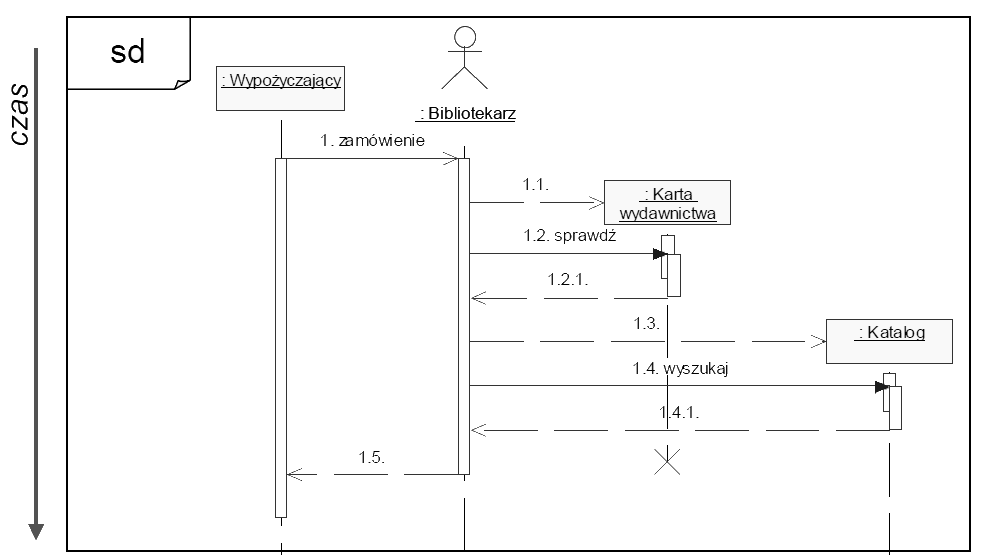
\includegraphics[width=\linewidth]{uml_sek.png}
    \end{figure}

    \subsection{Diagram przypadków użycia.}

    \begin{definition}
        \textbf{Diagram przypadków użycia} służy do przedstawiania:
        \begin{itemize}
            \item interakcji aktora z systemem,
            \item zadań, jakie wykonuje system,
            \item wymagań funkcjonalnych.
        \end{itemize}


        \textbf{Aktorzy} mogą być:
        \begin{itemize}
            \item Ludźmi wchodzącymi w interakcję,
            \item Systemami zewnętrznymi
            \item Częściami systemu, które mają wpływ na funkcjonowanie systemu, ale same przez ten system nie mogą
            być zmieniane (jak np. zegar systemowy).
        \end{itemize}
    \end{definition}

    \begin{figure}[H]
        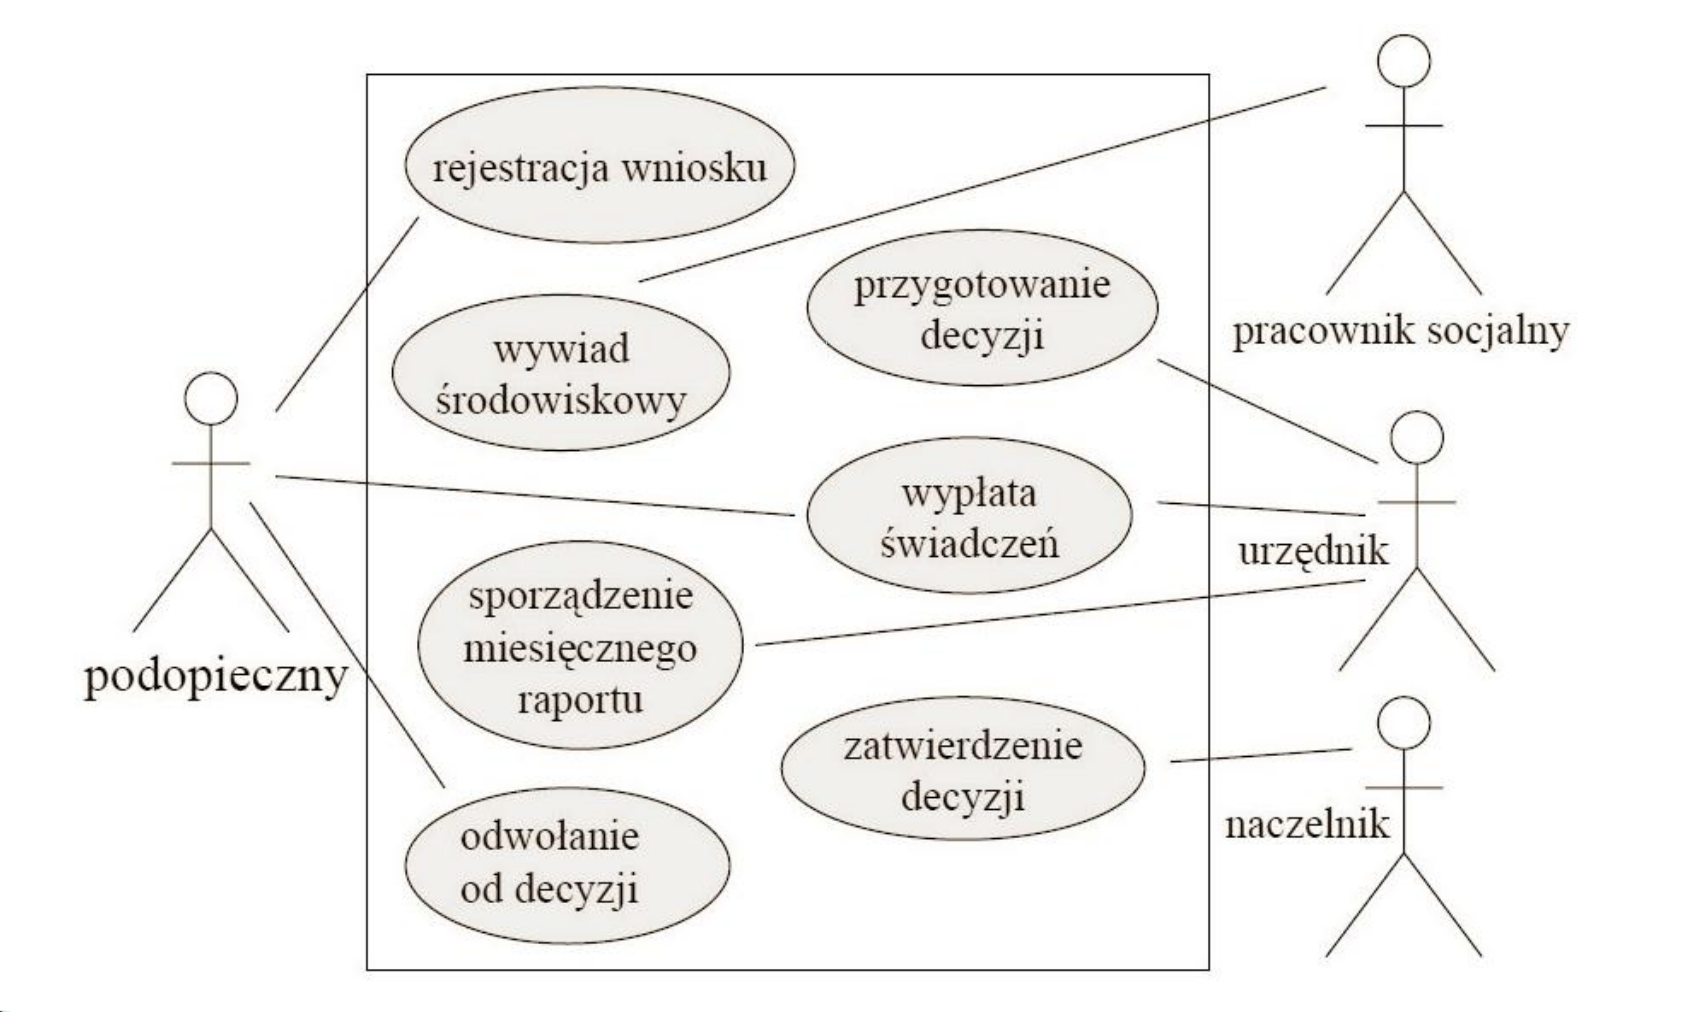
\includegraphics[width=\linewidth]{uml_pu.png}
    \end{figure}

    \newpage

    \section{Klasyfikacja testów.}

    \subsection{Poziomy testów.}
    \begin{definition}
        \textbf{Poziom testów} określa \textbf{sposób} testowania ze względu na \textbf{postać}
        testowanego obiektu w kontekście cyklu życia (\textbf{co testujemy?}).
    \end{definition}

    \subsubsection{Testy jednostkowe.}

    \begin{table}[H]
        \begin{center}
            \begin{tabular}{| p{4cm}| p{12cm}|}
                \hline
                \multicolumn{2}{|c|}{ \textbf{TESTY JEDNOSTKOWE}}\\
                \hline
                \textbf{Podstawa testów} & wymagania na moduły, projekt szczegółowy, kod\\
                \hline
                \textbf{Typowe obiekty} & moduły, programy, funkcje, klasy, procedury\\
                \hline
            \end{tabular}
        \end{center}
    \end{table}


    \begin{itemize}
        \item testowanie modułowe, unit testing
        \item defekty szukane w izolacji od reszty systemu
        \item wykorzystanie zaślepek i sterowników
        \item przeprowadzane przez deweloperów – autorów testowanego kodu
        \item usuwanie defektów bezpośrednio po znalezieniu
        \item brak formalnego procesu zarządzania defektami
    \end{itemize}

    \hfill \\

    \noindent \textbf{TTD} - Test Driven Developement.
    \begin{itemize}
        \item \textbf{Napisanie testu} - sprawdza, że programista rozumie zachowanie nowego kodu.
        \item \textbf{Uruchomienie testu}, który nie przechodzi (testuje uprząż testową i sam test; pokazuje,
        że wystąpi awaria, gdy kod będzie błędny).
        \item \textbf{Napisanie kodu} w minimalnej ilości, wystarczającej do zdania testu; jeśli
        konieczne, dokonanie refaktoryzacji.
    \end{itemize}

    \subsubsection{Testy integracyjne.}

    \begin{table}[H]
        \begin{center}
            \begin{tabular}{| p{4cm}| p{12cm}|}
                \hline
                \multicolumn{2}{|c|}{ \textbf{TESTY INTEGRACYJNE}}\\
                \hline
                \textbf{Podstawa testów} & projekt systemu, architektura, przypadki użycia\\
                \hline
                \textbf{Typowe obiekty} & interfejsy, podsystemy, konfiguracje systemów\\
                \hline
            \end{tabular}
        \end{center}
    \end{table}

    \begin{itemize}
        \item testuje interfejsy i interakcje
        \item im większy zakres integracji, tym trudniej izolować defekty
        \item rozumienie architektury testowanych modułów/systemów
        \item może odbywać się na wielu poziomach (np. integracja systemów)
    \end{itemize}

    \begin{figure}[H]
        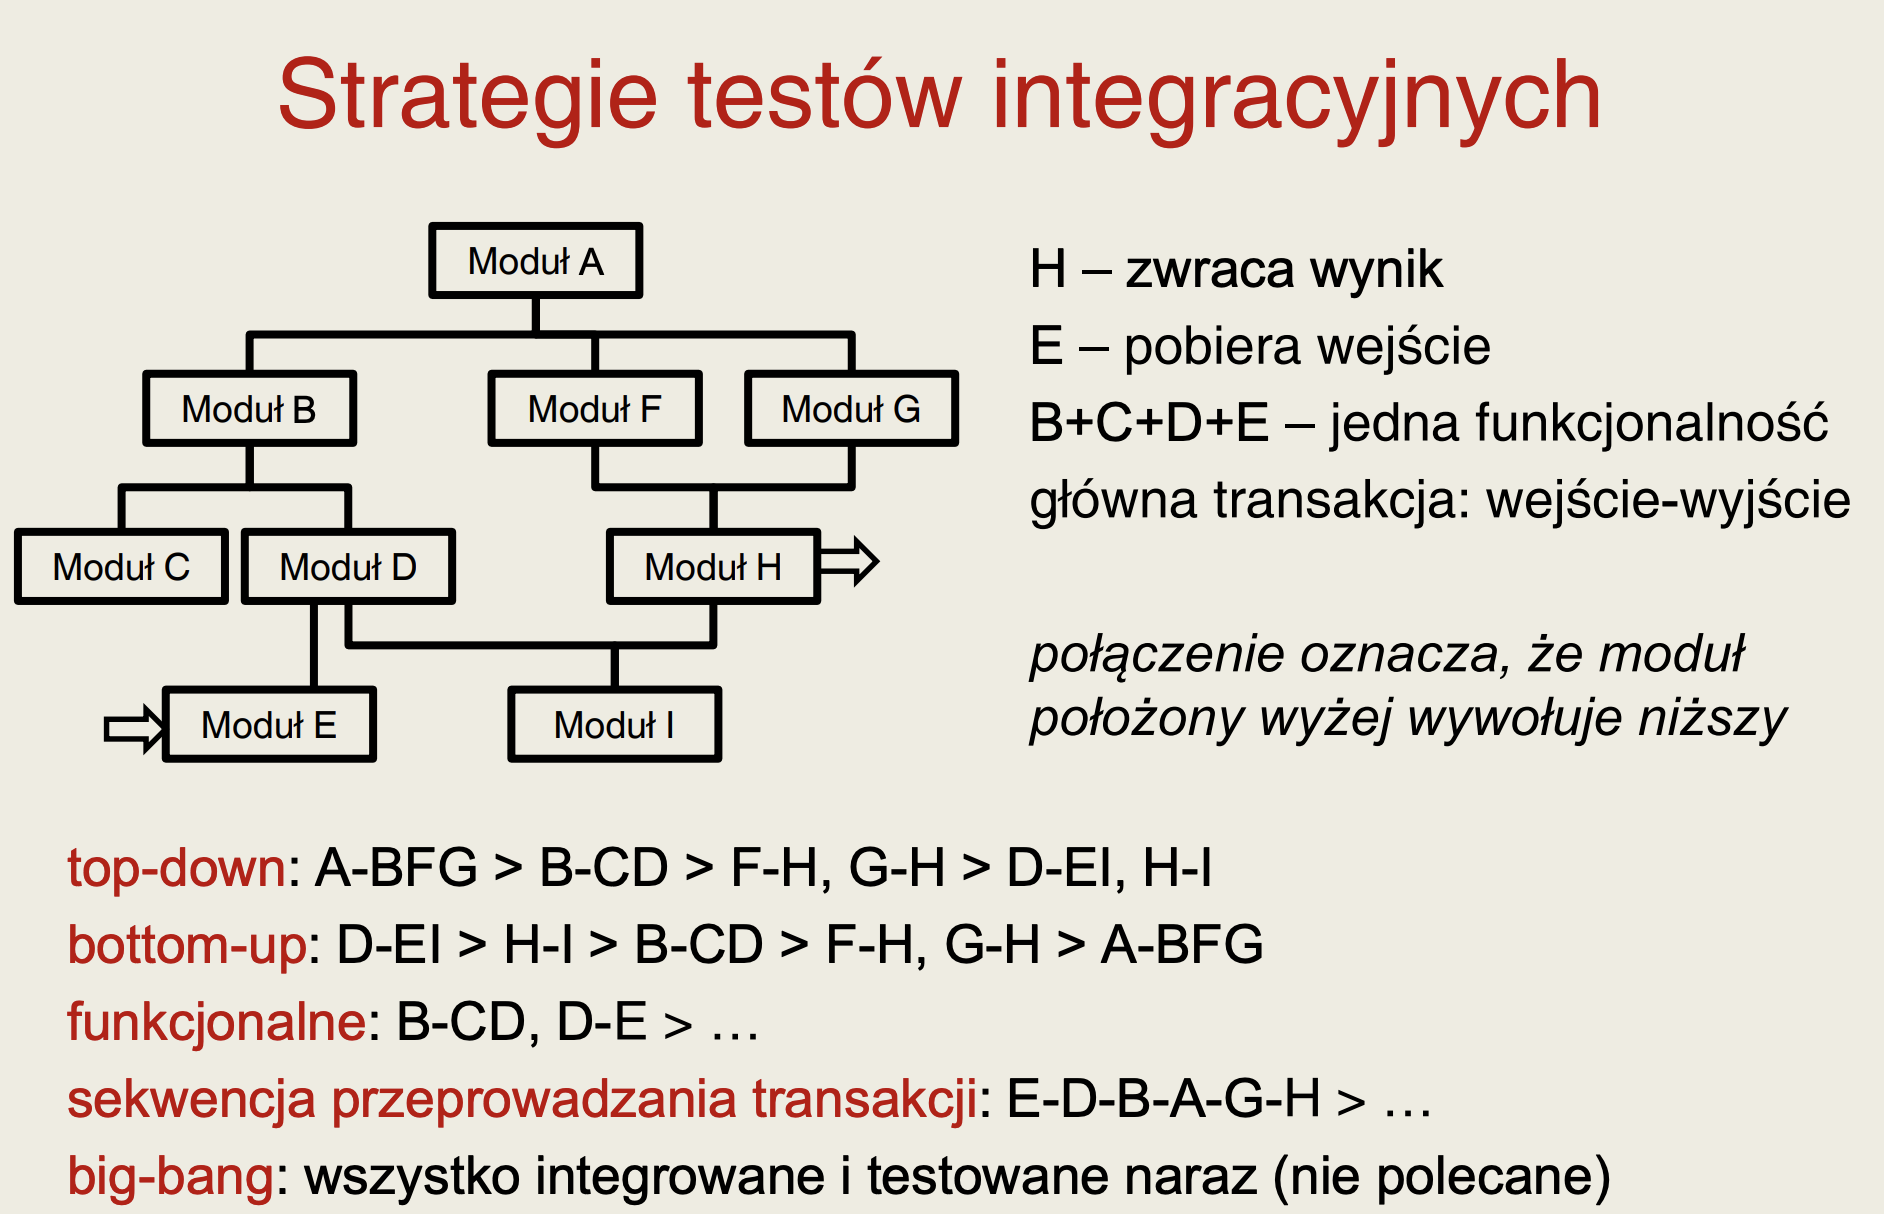
\includegraphics[width=\linewidth]{strat_integr.png}
    \end{figure}

    \subsubsection{Testy systemowe.}

    \begin{table}[H]
        \begin{center}
            \begin{tabular}{| p{4cm}| p{12cm}|}
                \hline
                \multicolumn{2}{|c|}{ \textbf{TESTY SYSTEMOWE}}\\
                \hline
                \textbf{Podstawa testów} & wymagania na system, przypadki użycia,
                specyfikacja funkcjonalna, raporty analizy ryzyka\\
                \hline
                \textbf{Typowe obiekty} & system, podręczniki użytkownika i operatora,
                konfiguracja systemu\\
                \hline
            \end{tabular}
        \end{center}
    \end{table}

    \begin{itemize}
        \item sprawdza zachowanie systemu jako całości
        \item zakres testu określony w planie testów
        \item środowisko testowe podobne do produkcyjnego – minimalizacja ryzyka awarii zależnych od środowiska
        \item często konieczność testowania z niekompletnymi wymaganiami
        \item zwykle przeprowadzane przez niezależny zespół testerski
    \end{itemize}

    \subsubsection{Testy akceptacyjne.}

    \begin{table}[H]
        \begin{center}
            \begin{tabular}{| p{4cm}| p{12cm}|}
                \hline
                \multicolumn{2}{|c|}{ \textbf{TESTY AKCEPTACYJNE}}\\
                \hline
                \textbf{Podstawa testów} & wymagania użytkownika, wymagania na system,
                przypadki użycia, procesy biznesowe, raporty
                analizy ryzyka\\
                \hline
                \textbf{Typowe obiekty} & Procesy biznesowe w pełni zintegrowanego
                systemu, procesy operacyjne i utrzymania systemu,
                procedury, raporty, dane konfiguracyjne\\
                \hline
            \end{tabular}
        \end{center}
    \end{table}

    \begin{itemize}
        \item cel: zyskanie zaufania do systemu
        \item znajdowanie defektów nie jest głównym celem
        \item często przeprowadzane przez klienta lub użytkownika
        \item ocenia gotowość systemu, ale niekoniecznie ostatni etap testów
    \end{itemize}

    \noindent \textbf{Typowe formy testów akceptacyjnych:}
    \begin{itemize}
        \item \textbf{testy akceptacyjne użytkownika (UAT)} – sprawdzenie gotowości do użycia
        \item \textbf{testy operacyjne (OAT)} – akceptacja przez administratora systemu (testy
        backupu, przywracania systemu, zarządzania użytkownikami, utrzymania,
        migracji danych, bezpieczeństwa itp.)
        \item \textbf{testy akceptacyjne wymagane kontraktem/regulacjami}
        \item \textbf{testy alfa, beta (polowe)}
        \begin{itemize}
            \item alfa: przeprowadzane u producenta, ale nie przez zespół deweloperski
            \item beta: przeprowadzane u klienta przez klienta/potencjalnego użytkownika
        \end{itemize}
    \end{itemize}

    \subsection{Typy testów.}

    \begin{definition}
        \textbf{Typ testów} to zbiór czynności testowych właściwych dla weryfikacji systemu
        w oparciu o konkretny powód lub cel testów (\textbf{jak testujemy?}).
    \end{definition}

    \begin{enumerate}
        \item  \textbf{Testowanie funkcjonalne}\\
        Testowanie funkcji wykonywanej przez oprogramowanie - \textbf{co system robi}.

        \item \textbf{Testowanie niefunkcjonalne}\\
        Testowanie niefunkcjonalnej charakterystyki jakościowej (np. niezawodność, wydajność,
        użyteczność) - \textbf{jak system działa}. Wyrażalne ilościowo (np. czas odpowiedzi w testach wydajności).

        \item \textbf{Testowanie strukturalne}\\
        Oparte na strukturze (np. kod, graf przepływu sterowania, struktura menu, model procesu biznesowego).
        Zwykle wykonywane po testach czarnoskrzynkowych, aby sprawdzić stopień przetestowania i wyrazić go ilościowo
        (\textbf{pokrycie}).

        \item \textbf{Retesty i testy regresji}\\
        \textbf{Związane ze zmianą}, tzn. potwierdzenie usunięcia defektów (retesty - testy zmienionych fragmentów kodu)
        oraz poszukiwanie niezamierzonych zmian (regresja - pogarszanie się jakości systemu przy wprowadzaniu zmian;
        testujemy niezmienione fragmenty programu- często automatyzowane).
    \end{enumerate}

    \newpage

    \section{Model Scrum: struktura zespołu, proces wytwarzania oprogramowania, korzyści modelu.}
    \begin{definition}
        \textbf{SCRUM} jest:
        \begin{itemize}
            \item lekki
            \item łatwy do zrozumienia
            \item bardzo trudny do opanowania
        \end{itemize}

        Teoria SCRUMa opiera się na trzech filarach:
        \begin{itemize}
            \item \textbf{Przejrzystość} - wszystkie istotne aspekty procesu muszą być widoczne dla osób odpowiedzialnych za osiągane rezultaty
            \item \textbf{Adaptacja} - powinna być ciągła. Korekta musi być wykonana jak najszybciej, by ograniczyć dalsze następstwa problemów
            \item \textbf{Inspekcja} - poddawane regularnej inspekcji są zarówno scrumowe artefakty jak i postępy prac
        \end{itemize}
    \end{definition}

    \subsection{Struktura zespołu}

    \begin{definition}
        \textbf{Struktura zespołu} \\
        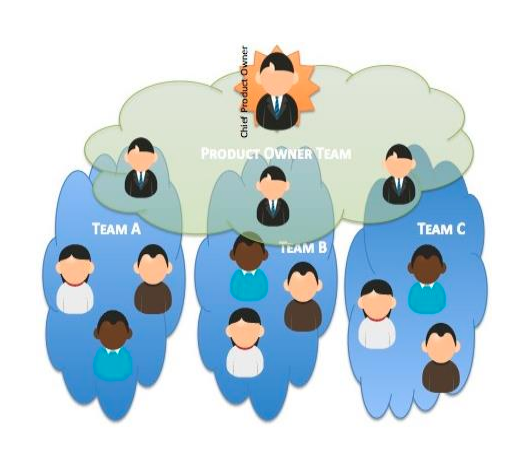
\includegraphics[width=\linewidth]{scrum_teams.png}
    \end{definition}

    \begin{definition}
        \textbf{Product owner} - jest odpowiedzialny za maksymalizację wartości produktu i pracy Zespołu Deweloperskiego. jest jedyną osobą zarządzającą Rejestrem Produktu (Product Backlog) co rozumiemy przez:
        \begin{itemize}
            \item Jasne artykułowanie elementów Rejestru Produktu i określanie ich kolejności w sposób zapewniający osiąganie założonych celów i misji
            \item Zapewnianie, że Rejestr Produktu jest dostępny, przejrzysty oraz jasny dla wszystkich i, że dobrze opisuje to, czym Zespół Scrumowy będzie się zajmował
        \end{itemize}
    \end{definition}

    \begin{definition}
        \textbf{Zespół Deweloperski}:
        \begin{itemize}
            \item Jest złożony z profesjonalistów
            \item Ma za zadanie dostarczenie (na zakończenie każdego Sprintu), gotowego do wydania Przyrostu produktu
            \item Zalecana liczebność: 3-9 osób
            \item Są samoorganizujące się
            \item Jest wielofunkcyjny, w swoim składzie posiadają wszystkie umiejętności niezbędne do wytworzenia Przyrostu
            \item Scrum nie przewiduje tytułów innych niż ``Deweloper'' dla członków Zespołu Deweloperskiego
            \item Odpowiedzialność za wykonywaną pracę ponosi cały Zespół Deweloperski; nie składają się z podzespołów
        \end{itemize}
    \end{definition}

    \begin{definition}
        \textbf{Scrum Master} - jest odpowiedzialny za to, by Scrum był rozumiany i stosowany. Scrum Masterzy dokonują tego poprzez upewnianie się,
        że Zespół Scrumowy stosuje się do założeń teorii Scruma, jego praktyk i reguł postępowania. Scrum Master wspiera zarówno Właściciela Produktu jak i zespól deweloperski.
    \end{definition}

    \subsection{Zdarzenia}

    \begin{definition}
        \textbf{Zdarzenia} \\
        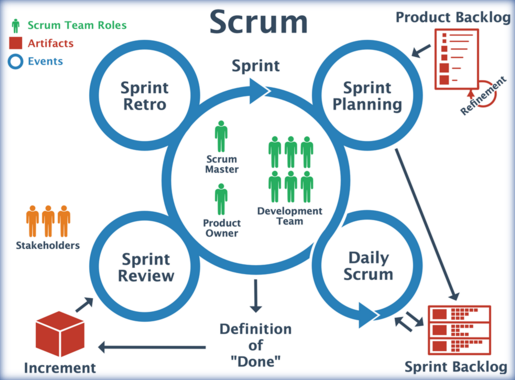
\includegraphics[width=\linewidth]{scrum_events.png}
    \end{definition}

    \begin{definition}
        \textbf{Planowanie sprintu} - planowanie co zostanie wykonane podczas najbliższego sprintu:
        \begin{itemize}
            \item Jest ograniczone czasowo (8h dla miesięcznego sprintu i proporcjonalnie)
            \item Planowanie Sprintu składa się z dwóch części:
            \begin{itemize}
                \item Co zostanie dostarczone
                \item Jaka praca zostanie wykonana
            \end{itemize}
        \end{itemize}
    \end{definition}

    \begin{definition}
        \textbf{Sprint} - serce SCUMa:
        \begin{itemize}
            \item Ograniczony czasowo - trwa miesiąc lub krócej
            \item Podczas Sprintu wytwarzany jest Przyrost „Ukończonej”, używalnej i potencjalnie gotowej do wydania funkcjonalności
            \item Ma stałą długość przez cały okres trwania prac
            \item Niedozwolone są zmiany, które wpłyną na cel Sprintu
            \item Skład Zespołu Deweloperskiego i jego cel jakościowy pozostają niezmienne
            \item Przerwanie sprintu:
            \begin{itemize}
                \item Tylko product owner ma prawo przerwać sprint
                \item Sprint może zostać przerwany, jeśli cel Sprintu się zdezaktualizuje
                \item Powinien zostać przerwany, jeśli kontynuowanie prac nie ma sensu w zaistniałych okolicznościach
                \item Przerwania Sprintów zużywają zasoby, ponieważ wszyscy muszą się przegrupować podczas kolejnego Planowania Sprintu, aby móc rozpocząć nowy
            \end{itemize}
        \end{itemize}
    \end{definition}

    \begin{definition}
        \textbf{Daily scrum} - jest spotkaniem ograniczonym czasowo do 15 minut, w którym każdy z członków zespołu wyjaśnia:
        \begin{itemize}
            \item Co zostało wykonane od ostatniego potkania
            \item Co zostanie wykonane przed kolejnym spotkaniem
            \item Jakie przeszkody stoją na drodze
        \end{itemize}
    \end{definition}

    \begin{definition}
        \textbf{Przegląd sprintu} - organizowany jest na zakończenie Sprintu w celu przeprowadzenia inspekcji Przyrostu i dostosowaniu, jeśli zajdzie taka potrzeba, Rejestru Produktu. \\
        Podczas Przeglądu Sprintu \textbf{Zespół Scrumowy} i \textbf{interesariusze} wspólnie omawiają to, co zostało ukończone w Sprincie. \\
        Może trwać maksymalnie 4h dla miesięcznego Sprintu.
    \end{definition}

    \begin{definition}
        \textbf{Retrospektywa Sprintu} - jest okazją dla zespołu Scrumowego do przeprowadzenia inspekcji swoich działań i opracowania planu usprawnień. Ma na celu:
        \begin{itemize}
            \item Sprawdzenie, co działo się w ostatnim Sprincie, biorąc pod uwagę ludzi, zależności, procesy i narzędzia
            \item Zidentyfikowanie i uporządkowanie istotnych elementów, które sprawdziły się w działaniu oraz tych, które kwalifikują się do poprawy
            \item Stworzenie planu wprowadzania w życie usprawnień sposobu wykonywania pracy przez Zespół Scrumowy
        \end{itemize}
    \end{definition}

    \subsection{Artefakty}

    \begin{definition}
        \textbf{Rejestr produktu} - uporządkowana lista tego co może być potrzebne w produkcie. Jest to jedyne źródło wymaganych zmian, które mają zostać wprowadzone.
        Odpowiedzialny z rejestr produktu jest Product owner.
    \end{definition}

    \begin{definition}
        \textbf{Rejestr sprintu} - podzbiór elementów Rejestru produktu. Jest to lista rzeczy do wykonania w danym sprincie rozszerzona dodatkowo o plan ich wykonania.
        Rejestr Sprintu definiuje pracę, jaką Zespół Deweloperski wykona by przekształcić elementy Rejestru Produktu w „Ukończony” Przyrost. \\
        Rejestr Sprintu należy tylko i wyłącznie do Zespołu Deweloperskiego.
    \end{definition}

    \begin{definition}
        \textbf{Przyrost} - suma wszystkich elementów Rejestru Produktu zakończonych podczas Sprintu i wszystkich Sprintów poprzednich. \\
        Na koniec Sprintu nowy Przyrost musi być ``Ukończony''.
    \end{definition}

    \newpage

    \section{Wymagania w projekcie informatycznym: klasyfikacja, źródła, specyfikacja, analiza.}

    \begin{definition}
        \textbf{Wymagania} - opis funkcji (usług), które mają być realizowane przez system i opis ograniczeń dla systemu. \\
        Wymagania nie opisują jak system ma działać a co ma wykonywać.
    \end{definition}

    \subsection{Klasyfikacja}

    \begin{definition}
        Wymagania dzielimy na:
        \begin{itemize}
            \item \textbf{Funkcjonalne} - opisują jakie funkcje powinien mieć system, np. ``wprowadzanie nowej faktury'' lub ``generowanie raportu miesięcznego''
            \item \textbf{Pozafunkcjonalne} - opisują najczęściej pewne własności danych funkcjonalności, np. ``minimum 20 faktur na godzinę'', ``średni czas między awariami 2000000h'', itp.
        \end{itemize}
    \end{definition}

    \begin{definition}
        \textbf{Klasyfikacja atrybutów jakości oprogramowania}
        \begin{itemize}
            \item \textbf{F}unctionality - funkcjonalność
            \item \textbf{U}sability – użyteczność
            \item \textbf{R}eliability – niezawodność
            \item \textbf{P}erformance – wydajność
            \item \textbf{S}ecurity - bezpieczeństwo
        \end{itemize}
        w skrócie \textbf{FURPS}
    \end{definition}

    \subsection{Źródła}

    \begin{definition}
        \textbf{System powinien…} \\
        Jest to sposób spisywania wymagań w stylu: ``System powinien umożliwić wystawianie faktur'', ``System powinien generować zestawienie miesięczne faktur'', ``Faktura powinna zawierać co najmniej jedną pozycję''. \\

        Zalety:
        \begin{itemize}
            \item Łatwość spisywania
        \end{itemize}

        Wady:
        \begin{itemize}
            \item Słaba czytelność
            \item Trudne sprawdzanie kompletności, spójności
        \end{itemize}

        Obecnie nie używany
    \end{definition}


    \begin{definition}
        \textbf{Funkcje systemu} \\
        Polega na opisywaniu poszczególnych funkcji systemu. Analogicznie do funkcji matematycznych, każda funkcja systemu informatycznego ma swoje wejście, wyjście, efekty uboczne. \\
        Przykładowo, rozpatrując funkcję wystawiania faktury, wejściem mogą być pozycje faktury, wyjściem wydruk faktury (lub wysłanie jej faksem), natomiast efektem ubocznym zapisanie tej faktury w rejestrze faktur. \\

        Wady:
        \begin{itemize}
            \item Słaba czytelność
            \item Trudne do zrozumienia
        \end{itemize}

        Obecnie nie używany
    \end{definition}


    \begin{definition}
        \textbf{Przypadki użycia} \\
        Przykład: \\

        \textbf{UC1: Wystawianie faktury} \\
        \textbf{Atrybuty:} \\
        \textbf{Główny aktor: Użytkownik} \\
        \textbf{Priorytet: Wysoki} \\
        \textbf{Źródło: Łukasz Olek} \\

        \textbf{Główny scenariusz:} \\
        1. Sprzedawca pragnie wystawić fakturę. \\
        2. Sprzedawca wpisuje pozycje faktury. \\
        3. System podlicza fakturę, nadaje jej nowy numer i zapisuje w rejestrze. \\
        4. Sprzedawca drukuje fakturę. \\
        \textbf{Rozszerzenia:} \\
        3.A. Sprzedawca nie dodał żadnej pozycji \\
        3.A.1. System prosi o ponowne wprowadzenie pozycji (powrót do 2.) \\

        Zalety:
        \begin{itemize}
            \item Łatwość spisywania
            \item Czytelność
            \item Łatwość zrozumienia i wyobrażenia sobie przyszłego systemu
        \end{itemize}

        Jako mapę łączącą pojedyncze przypadki użycia można potraktować diagram przypadków użycia (UML).
    \end{definition}


    \begin{definition}
        \textbf{Historyjki użytkownika} \\

        \textbf{Who? What? Why?} \\

        Wzór: \\

        \textbf{jako} - osoba, przypisana rola \\
        \textbf{chcę} - cecha, funkcjonalność, czynność \\
        \textbf{ponieważ} - uzasadnienie, rezultat, korzyść \\
    \end{definition}

    \subsection{Analiza}

    \begin{definition}
        Celem analizy wymagań jest stworzenie modelu systemu, zwanego modelem analitycznym. Wysiłek uczestników projektu skupia się na strukturalizowaniu i formalizowaniu zabranych wcześniej wymagań. \\
        Inaczej mówiąc po przeanalizowaniu przez nas zebranych wymagań musimy to przełożyć na diagramy UML.
    \end{definition}

    \begin{definition}
        \textbf{Model analityczny} - reprezentuje tworzony system z perspektywy użytkownika; opis co system powinien robić
    \end{definition}

    \begin{definition}
        \textbf{Analityczny model obiektowy} (diagramy klas) - odzwierciedla indywidualne koncepcje korzystania z systemu, ich właściwości i relacje między nimi
    \end{definition}

    \begin{definition}
        \textbf{Model dynamiczny} (diagramy sekwencji i stanów) - koncentruje się na zachowaniu systemu
    \end{definition}

    \newpage

    \section{Analiza obiektowa: modele obiektowe i dynamiczne, obiekty encjowe, brzegowe i sterujące.}

    \subsection{Diagram klas}

    Diagram klas ma za zadanie:
    \begin{itemize}
        \item przedstawić strukturę systemu w modelach obiektowych poprzez
        ilustrację struktury klas i zależności między nimi
        \item przedstawić podział odpowiedzialności pomiędzy klasy systemu
        i rodzaj wymienianych pomiędzy nimi komunikatów
    \end{itemize}

    \begin{center}
        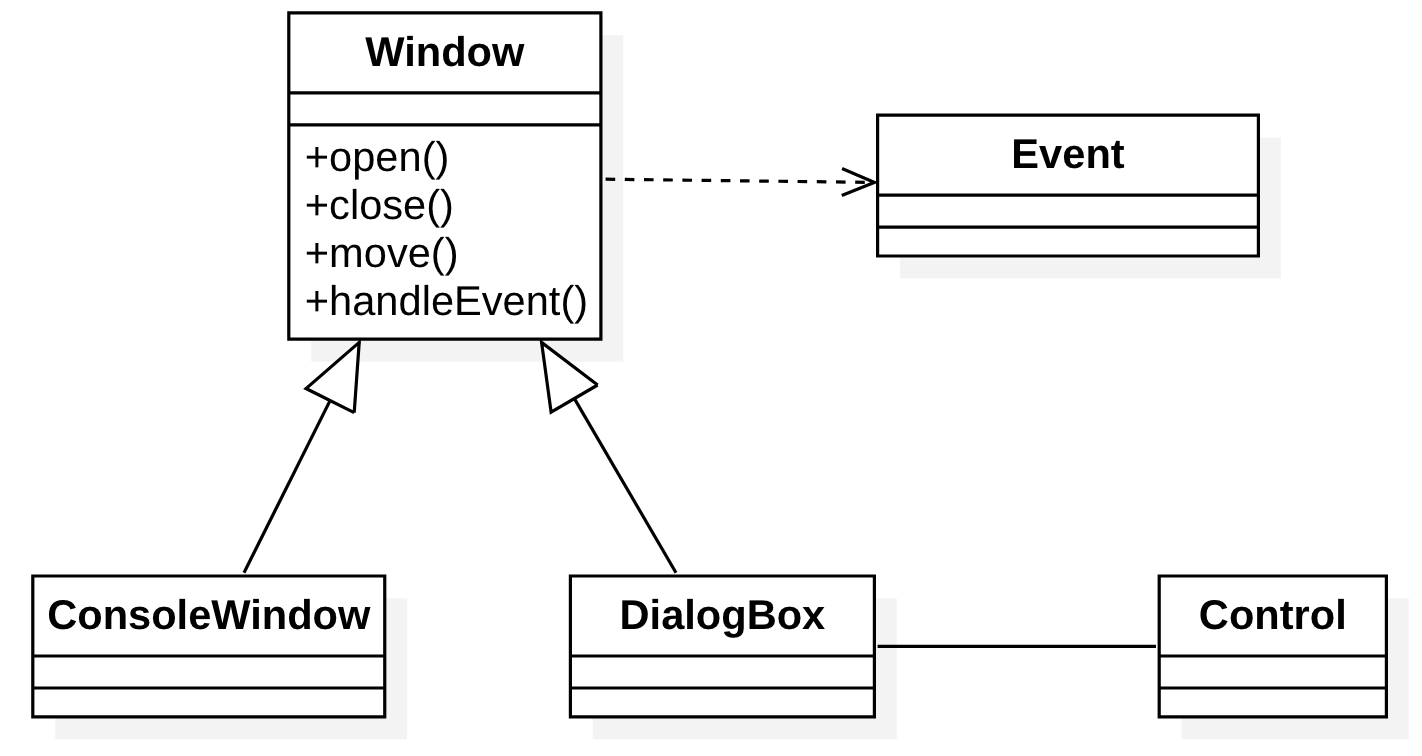
\includegraphics[scale=0.40]{ooad/uml.png}
    \end{center}


    \subsubsection{Klasy}

    Podstawowa część diagramu klas. Służą m.in. do opanowania słownictwa
    tworzonego systemu.

    Klasa składa się z:
    \begin{enumerate}
        \item Nazwy
        \item Atrybutów - czyli nazwanych właściwości klasy
        \item Operacji - implementacji pewnej usługi, której można żądać
        od obiektów klasy
        \item Odpowiedzialności (opcjonalnie)
    \end{enumerate}

    \begin{center}
        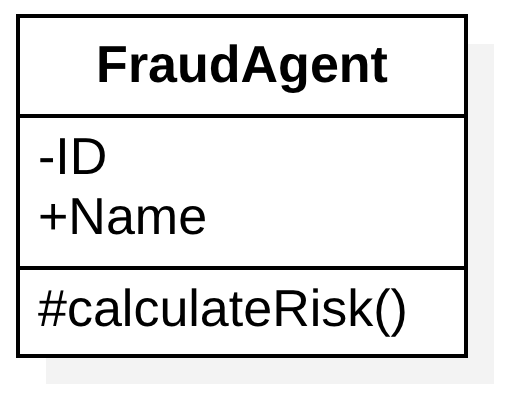
\includegraphics[scale=0.40]{ooad/class.png}
    \end{center}

    \subsubsection{Widoczność pól}

    \begin{itemize}
        \item \textbf{+} public
        \item \textbf{-} private
        \item \textbf{\#} protected
        \item \textbf{\~} package
    \end{itemize}

    \subsubsection{Związki}

    \begin{itemize}
        \item Asocjacja

        \begin{center}
            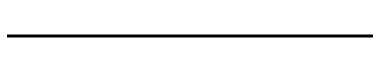
\includegraphics[scale=0.40]{ooad/association.png}
        \end{center}

        \item Zależność

        Informuje nas, że klasa używa innej klasy. Przykład:
        EventHandler i Event.
        \begin{center}
            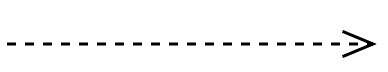
\includegraphics[scale=0.40]{ooad/dependency.png}
        \end{center}

        \item Generalizacja

        Czyli dziedziczenie lub uogólnienie. Określa zależność
        między klasą pochodną a klasą bazową.
        \begin{center}
            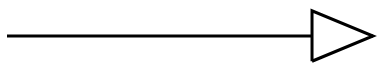
\includegraphics[scale=0.40]{ooad/generalization.png}
        \end{center}

        \item Realizacja

        Określa zależność między implementacją a interfejsem.
        Przykład: ArrayList i List.

        \begin{center}
            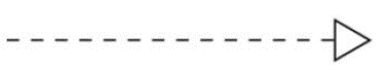
\includegraphics[scale=0.40]{ooad/realization.png}
        \end{center}

        \item Agregacja

        Określa zależność między częścią a całością.
        Przykład: cegła i mur.

        \begin{center}
            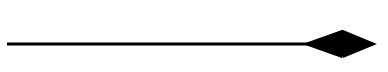
\includegraphics[scale=0.40]{ooad/composition.png}
        \end{center}

        \item Kompozycja

        Zwana również silną agregacją. Tak jak agregacja, określa
        zależność między częścią a całością, jednak część nie może
        istnieć bez całości. Przykład: wydział i uczelnia.

        \begin{center}
            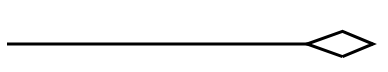
\includegraphics[scale=0.40]{ooad/aggregation.png}
        \end{center}
    \end{itemize}

    \newpage
    \subsection{Modele dynamiczne}

    \subsubsection{Diagram stanów}

    W UML dynamiczne aspekty systemu modeluje się za pomocą maszyny stanów.
    Diagram stanów zapewnia graficzną reprezentację stanów, przejść, zdarzeń i akcji.
    Notacja ta pozwala zwizualizować zachowanie obiektu w sposób, który pozwala
    podkreślić ważne elementy życia tego obiektu.

    \begin{center}
        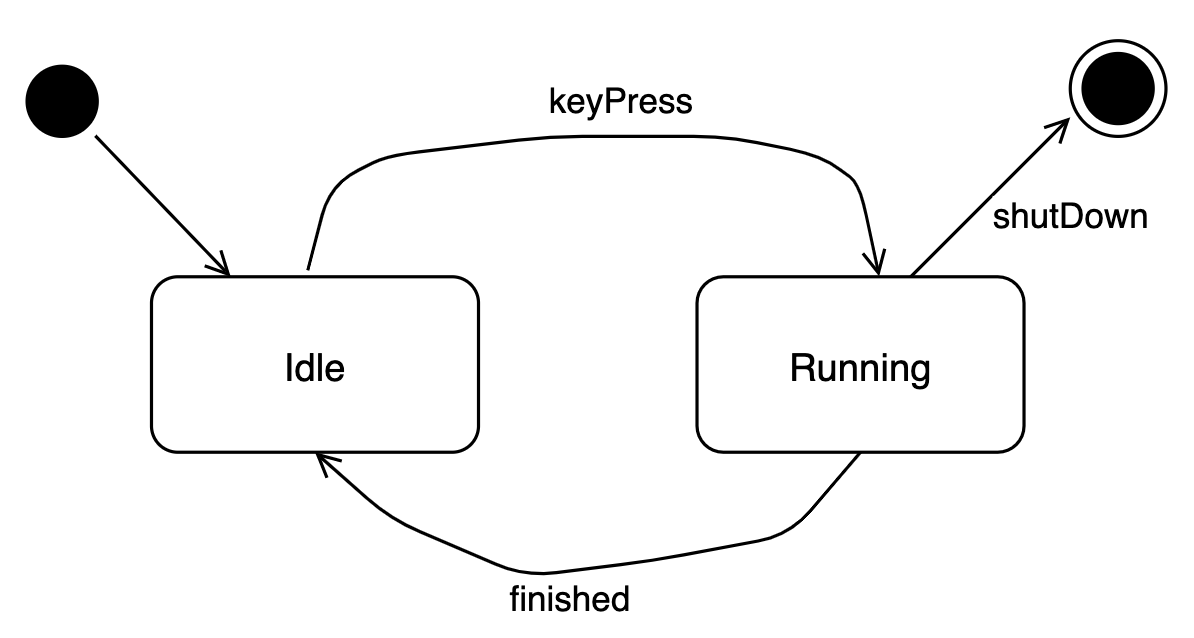
\includegraphics[scale=0.50]{state-diagram/diagram.png}
    \end{center}


    \begin{itemize}
        \item \textbf{Stan}

        Stan na diagramie reprezentuje sytuację lub stan obiektu,
        w którym spełnia on pewien warunek, wykonuje jakąś czynność lub czeka
        na jakieś zdarzenie. Obiekt pozostaje w stanie przez określony czas.
        Graficznie stan reprezentowany jest jako prostokąt z zaokrąglonymi narożnikami.

        \begin{center}
            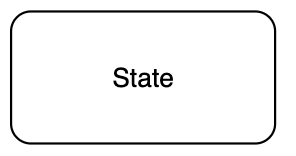
\includegraphics[scale=0.35]{state-diagram/state.png}
        \end{center}

        \newpage

        \begin{itemize}
            \item Podstany

            Możliwe jest podzielenie stanu na wewnętrzne podstany,
            z wewnętrznymi przejściami, akcjami, itp.

            \begin{center}
                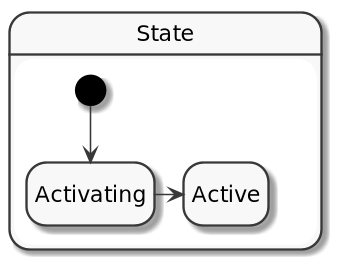
\includegraphics[scale=0.60]{state-diagram/substate.png}
            \end{center}

            \item Stan początkowy

            Wskazuje domyślne miejsce początkowe dla danego stanu lub automatu.
            Stan początkowy jest reprezentowany jako wypełnione czarne kółko.
            \begin{center}
                
\includegraphics[scale=0.40]{state-diagram/begin.png}
            \end{center}

            \item Stan końcowy

            Wskazuje, że wykonanie automatu stanów lub danego stanu zostało
            zakończone. Stan końcowy jest reprezentowany jako wypełnione
            czarne koło otoczone niewypełnionym okręgiem.

            \begin{center}
                
\includegraphics[scale=0.40]{state-diagram/end.png}
            \end{center}

        \end{itemize}

        \newpage

        \item \textbf{Przejścia}


        Przejście to związek między dwoma stanami wskazujący, że obiekt
        w pierwszym stanie wykona określone działania i przejdzie w drugi
        stan, gdy wystąpi określone zdarzenie i spełnione zostaną
        określone warunki.

        \begin{itemize}
            \item Zdarzenia

            Wystąpienie bodźca, który może wywołać zmianę stanu.

            \begin{center}
                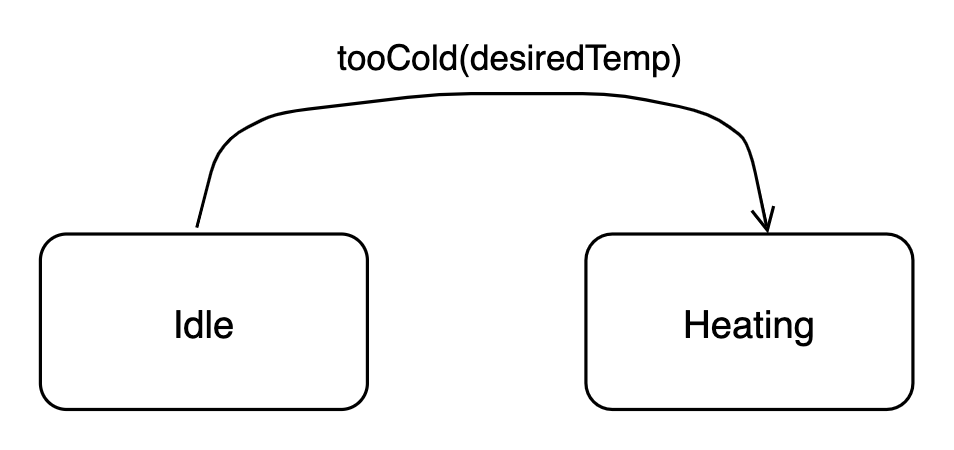
\includegraphics[scale=0.50]{state-diagram/event.png}
            \end{center}


            \item Akcje

            Wykonywalne obliczenie atomowe. Akcje mogą obejmować wywołania
            operacji (do obiektu będącego właścicielem maszyny stanu, a także
            do innych widocznych obiektów), utworzenie lub zniszczenie innego
            obiektu lub wysłanie sygnału do obiektu. Istnieje specjalny zapis
            do wysyłania sygnału - nazwa sygnału jest poprzedzona słowem
            kluczowym send jako wskazówką wizualną.

            \begin{center}
                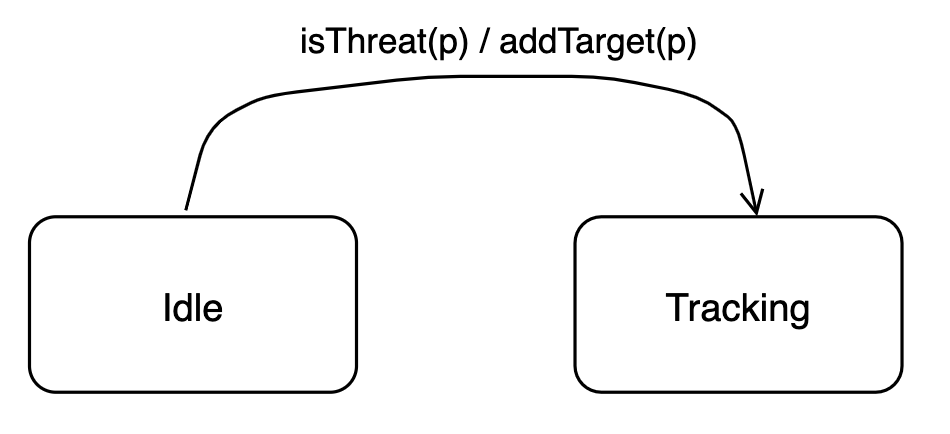
\includegraphics[scale=0.50]{state-diagram/action.png}
            \end{center}

            \begin{center}
                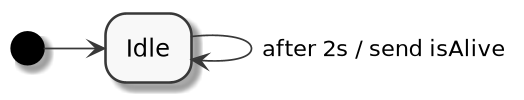
\includegraphics[scale=0.50]{state-diagram/signal.png}
            \end{center}

        \end{itemize}
    \end{itemize}

    \subsubsection{Diagram sekwencji}

    Diagram ten opisuje interakcje pomiędzy częściami systemu w postaci sekwencji
    komunikatów wymienianych między nimi. Ukazuje dynamiczne aspekty realizacji
    scenariuszy, w których dochodzi do złożonych oddziaływań pomiędzy obiektami

    \begin{center}
        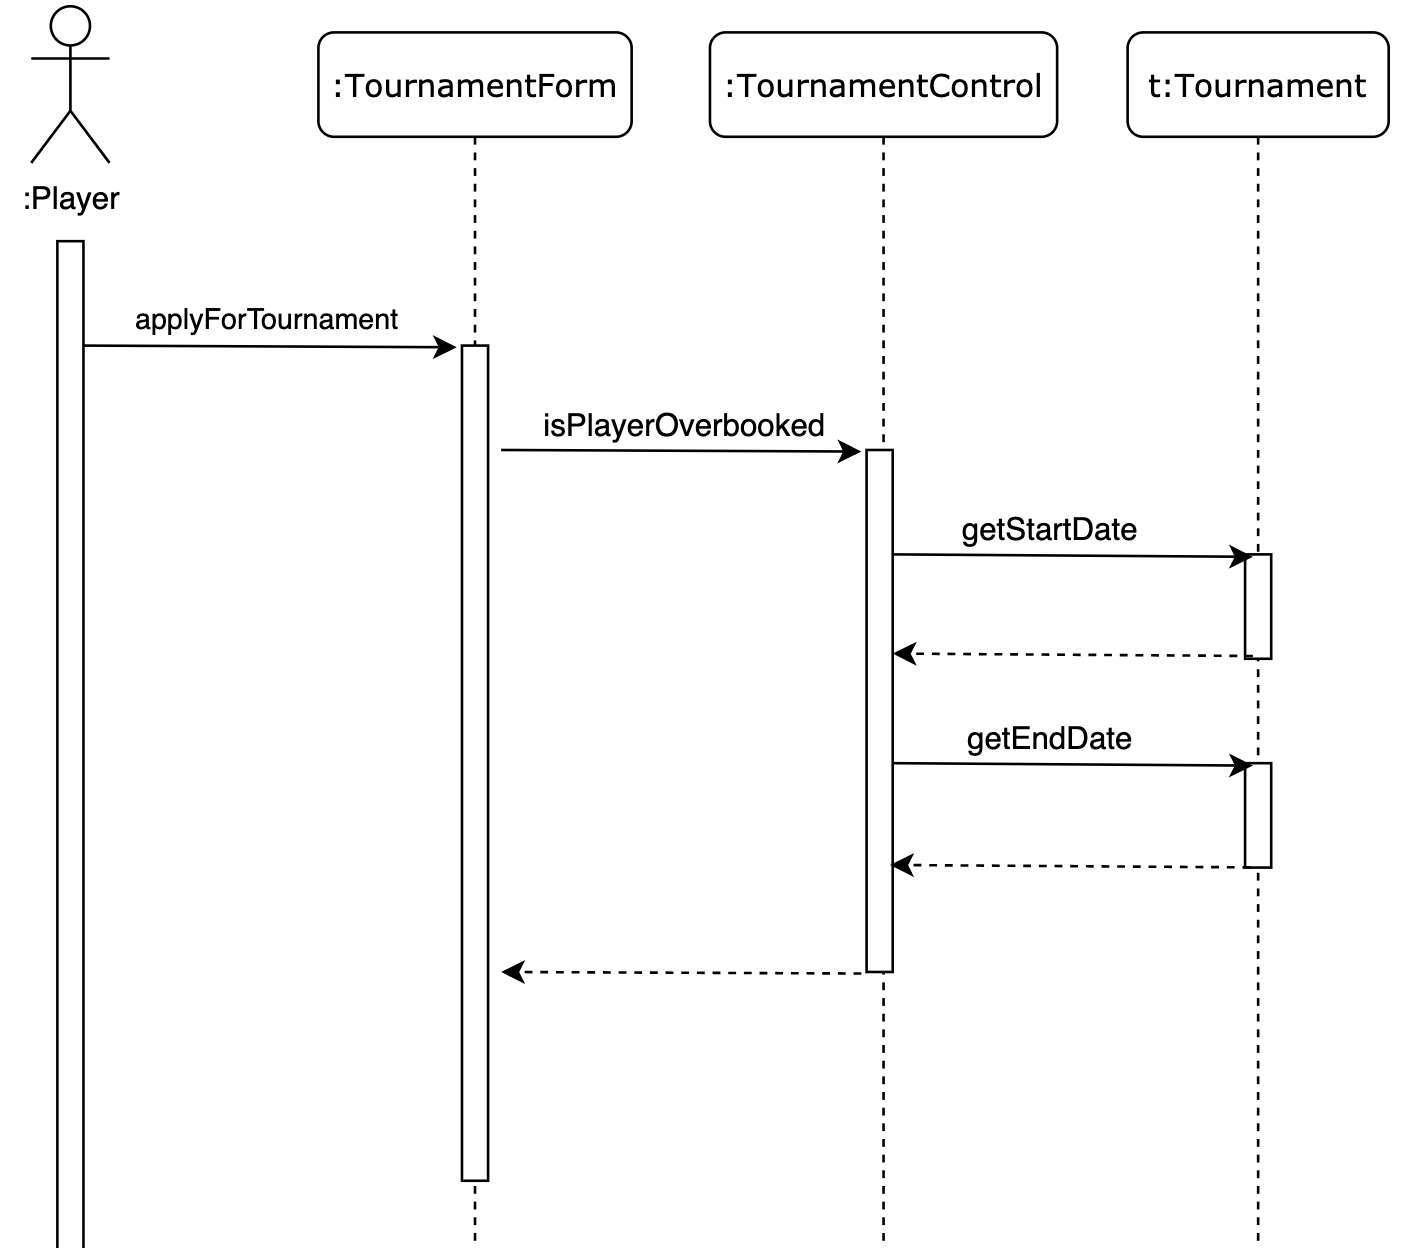
\includegraphics[scale=0.40]{ooad/sequence.png}
    \end{center}

    Rodzaje komunikatów:

    \begin{itemize}
        \item Wywołanie funkcji

        \begin{center}
            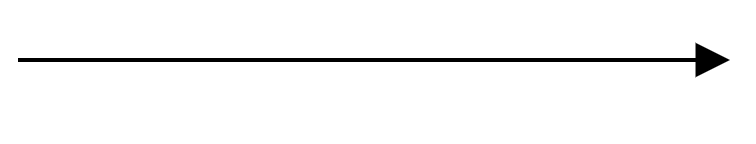
\includegraphics[scale=0.35]{ooad/normal.png}
        \end{center}

        \item Powrót z wywołania

        \begin{center}
            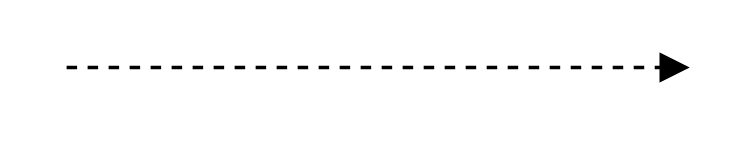
\includegraphics[scale=0.40]{ooad/return.png}
        \end{center}

        \item Wywołanie asynchoniczne

        \begin{center}
            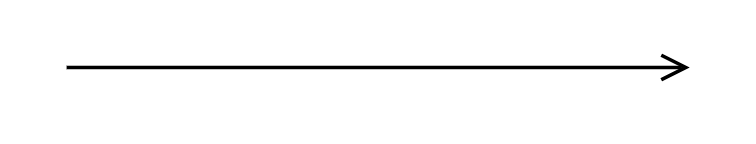
\includegraphics[scale=0.40]{ooad/async.png}
        \end{center}

    \end{itemize}

    \subsection{Encja-Brzeg-Sterowanie}

    Model ten dzieli obiekty wchodzące w ramy systemu na trzy typy:
    \begin{itemize}
        \item \textbf{Obiekty encji}

        Reprezentują trwałą informację przetwarzaną przez system

        \item \textbf{Obiekty brzegowe}

        Odzwierciedlają interakcje między aktorami a systemem

        \item \textbf{Obiekty sterujące}

        Odpowiadają za realizację przypadków użycia

    \end{itemize}

    \begin{center}
        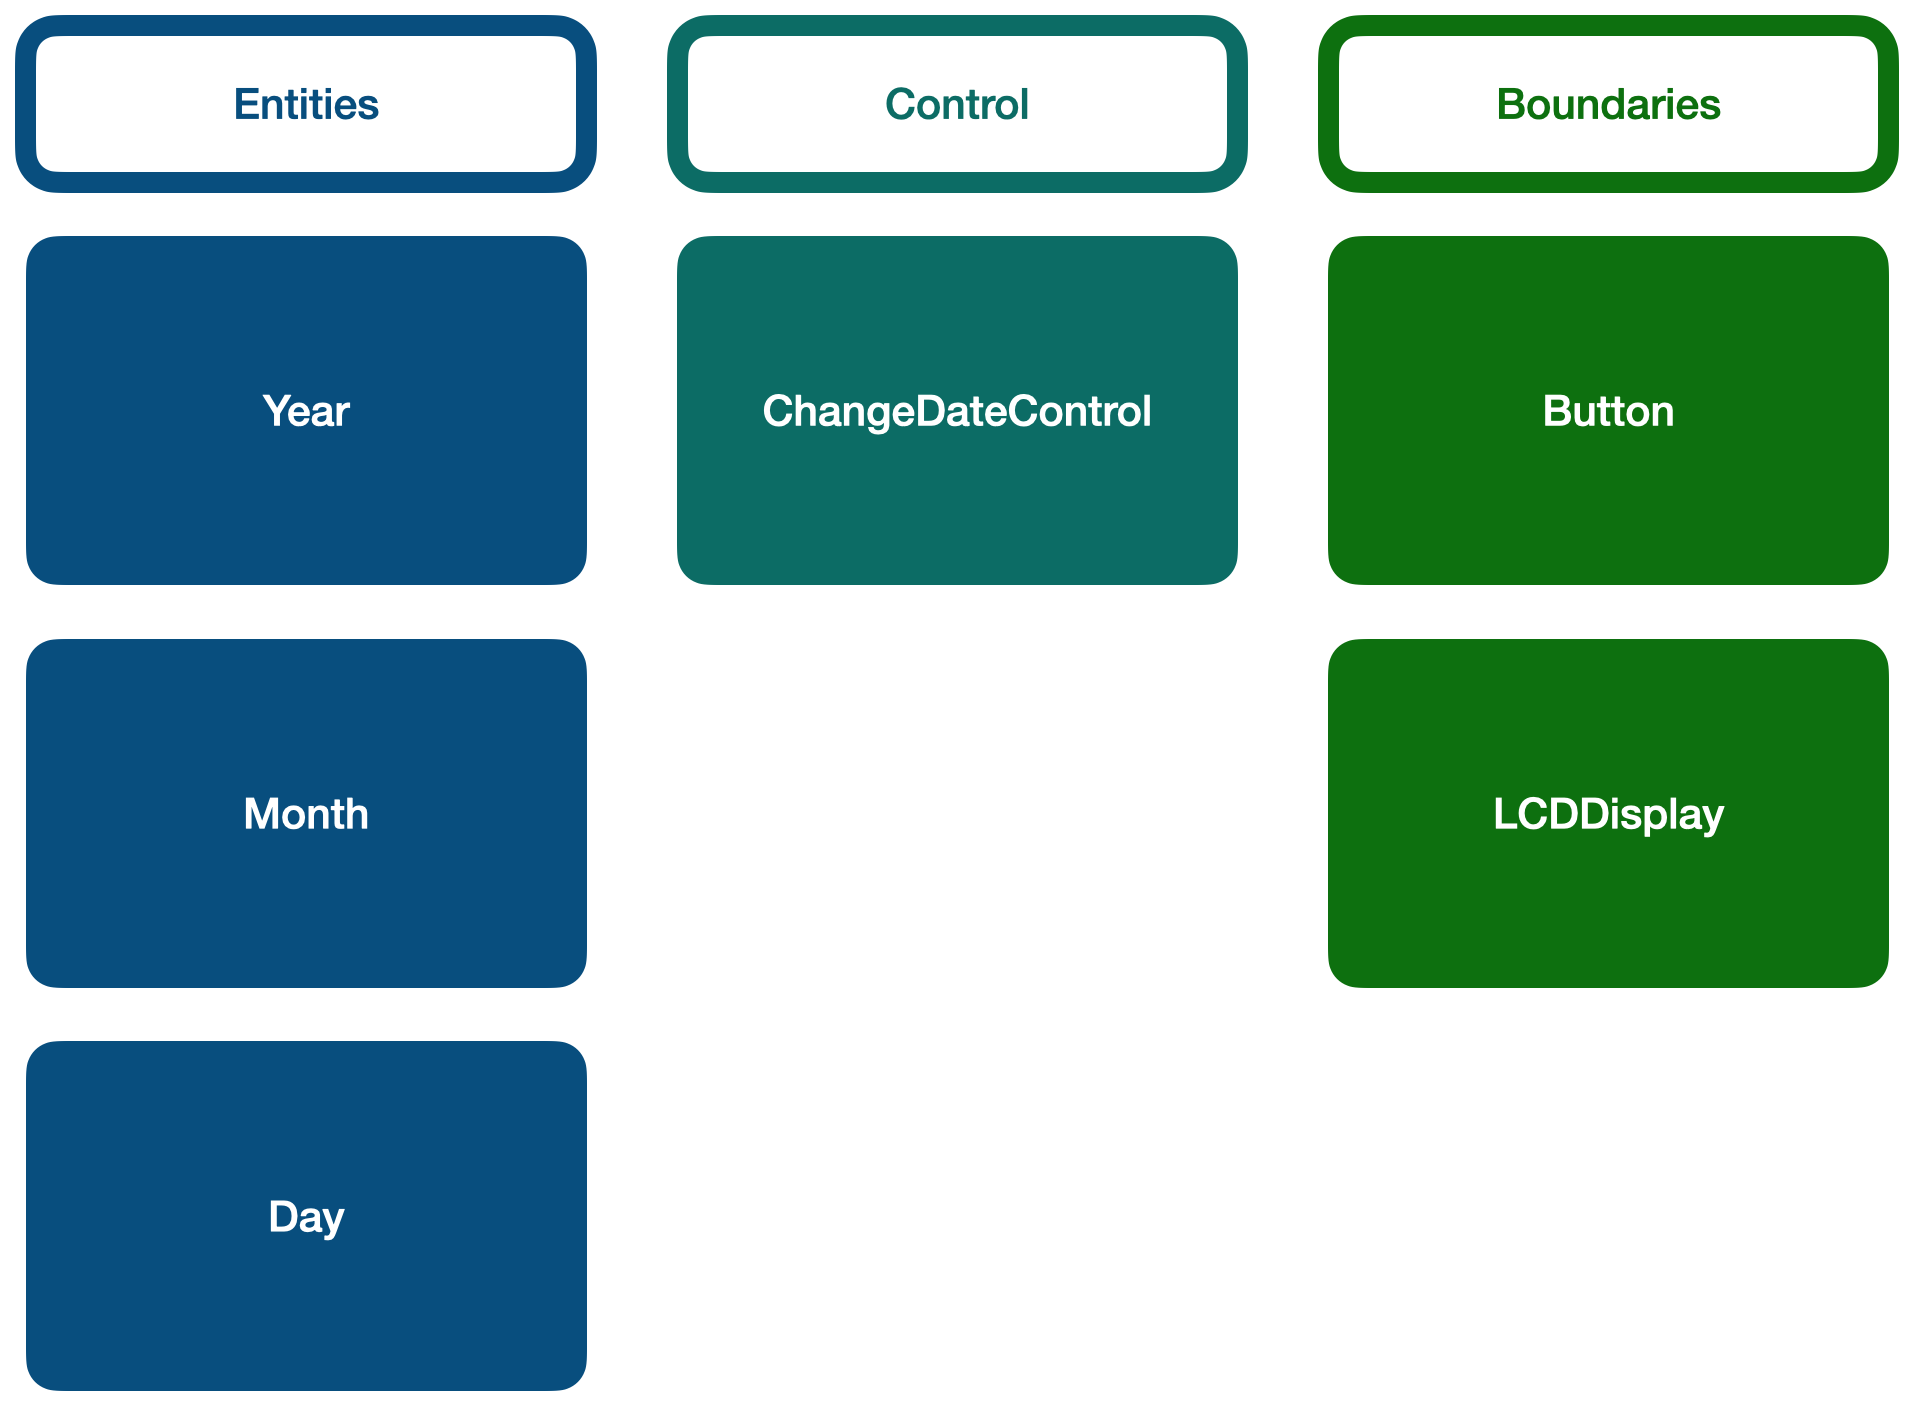
\includegraphics[scale=0.40]{ooad/ecb.png}
    \end{center}

    \begin{center}
        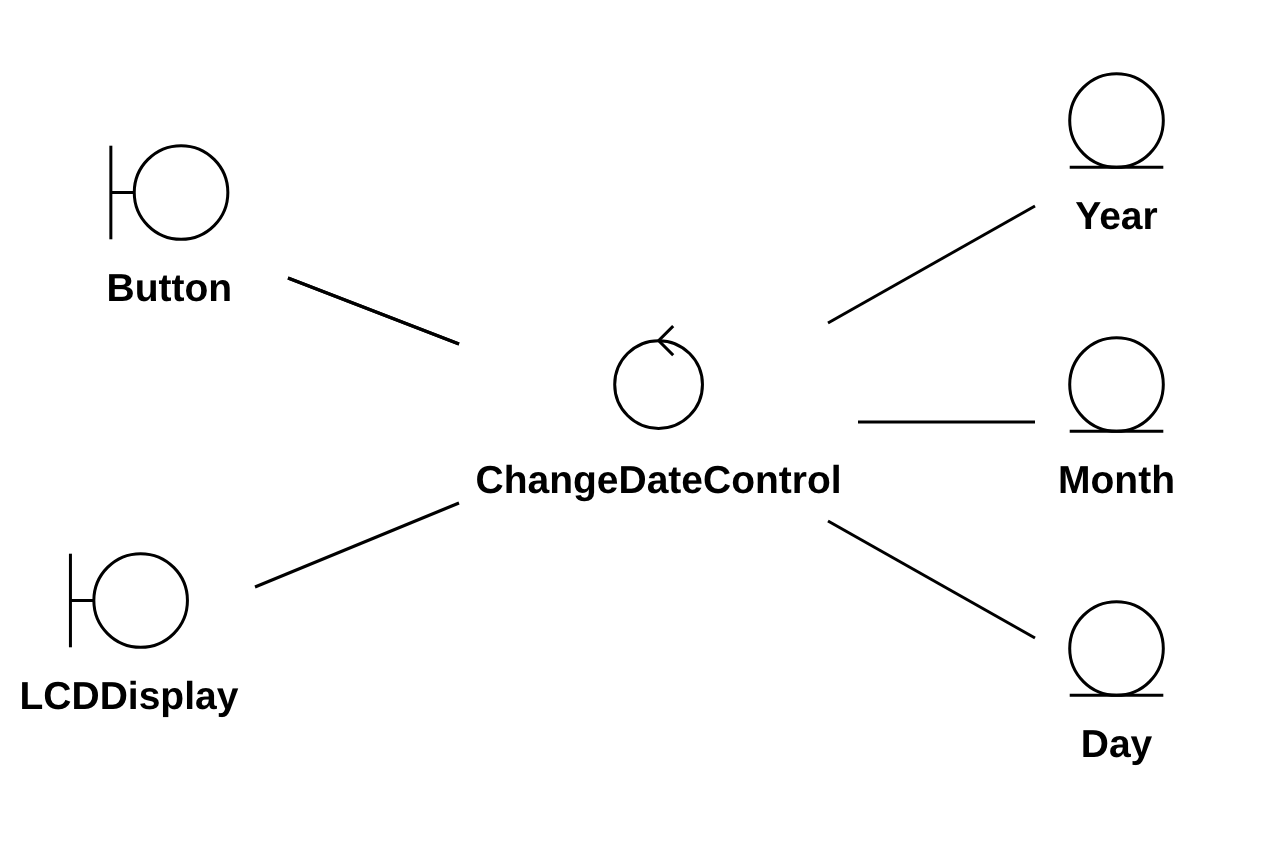
\includegraphics[scale=0.50]{ooad/ecb-uml.png}
    \end{center}
    \newpage

    \section{Wzorce architektury systemów.}

    \subsection{Architektura warstwowa}

    Efektem dekompozycji hierarchicznej jest
    uporządkowany zbiór warstw. Warstwa stanowi
    zgrupowanie podsystemów oferujących
    powiązane usługi.

    Wyróżniamy dwa rodzaje architektury warstwowej:
    otwartą i zamkniętą.

    Zalety:
    \begin{itemize}
        \item modyfikowalność
        \item prostota wykorzystania warstwy
        \item spójność i przejrzystość
        \item wielokrotne wykorzystanie
        \item naturalna ewolucja z tradycyjnego modelu aplikacji
    \end{itemize}

    \subsubsection{Architektura otwarta}

    W otwartej architekturze warstwowej warstwa może wywołać
    dowolną z warstw poniżej niej.

    \begin{center}
        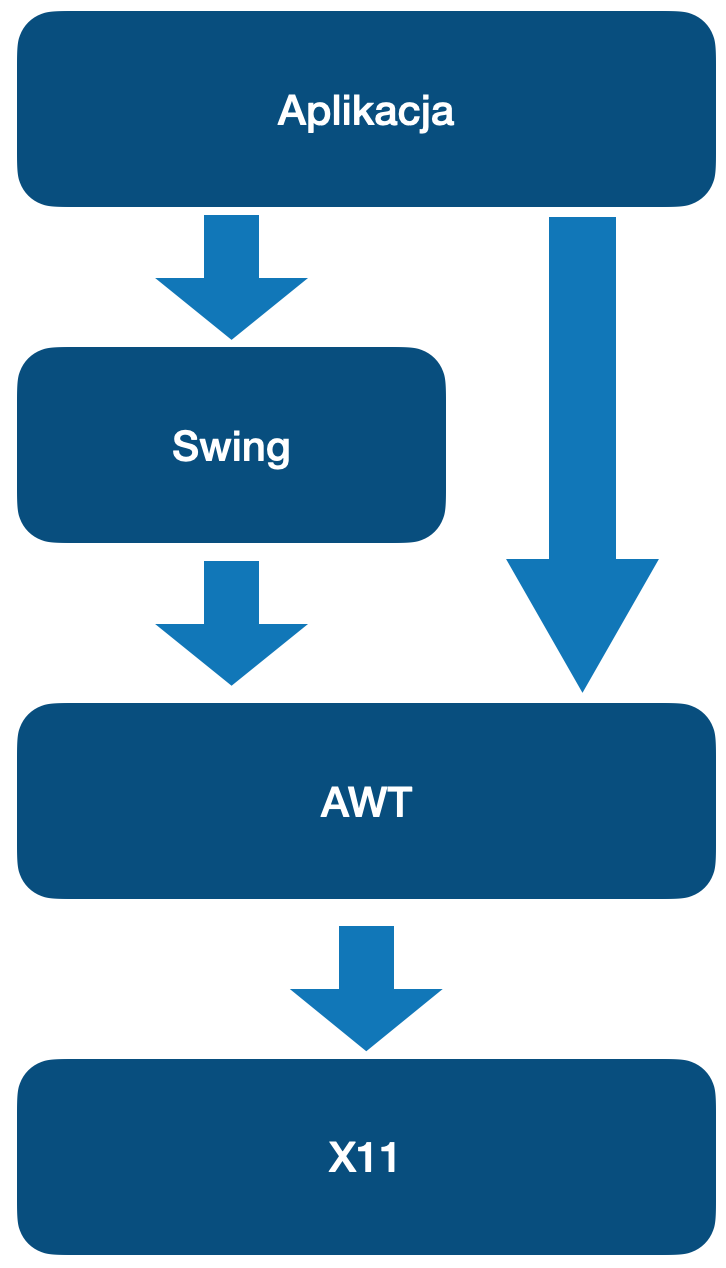
\includegraphics[scale=0.30]{patterns/swing.png}
    \end{center}

    Przykłady:
    \begin{itemize}
        \item Serverless
        \item Swing
    \end{itemize}

    \subsubsection{Architektura zamknięta}

    W zamkniętej architekturze warstwa może wywołać tylko warstwę
    bezpośrednio pod nią

    \begin{center}
        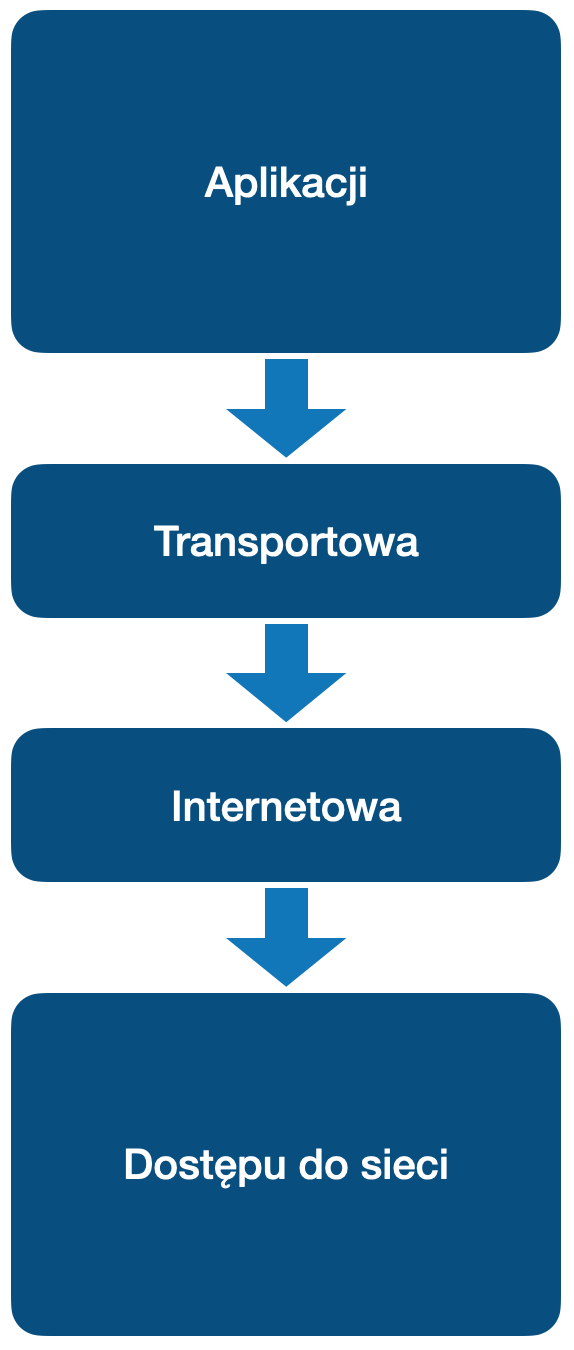
\includegraphics[scale=0.30]{patterns/tcp.png}
    \end{center}

    Przykłady:
    \begin{itemize}
        \item ISO/OSI
        \item TCP/IP
    \end{itemize}

    \subsubsection{Architektura trójwarstwowa}

    Architektura trójwarstwowa to architektura typu klient-serwer,
    często stosowana przy tworzeniu aplikacji internetowych.

    Warstwy:
    \begin{enumerate}
        \item Warstwa prezentacji

        Interfejs użytkownika. Tłumaczy żądania i wyniki
        do i z języka zrozumiałego dla użytkownika.

        \item Warstwa logiki biznesowej

        Koordynuje pracę aplikacji, przetwarza żądania
        warstwy prezentacji, dokonuje obliczeń.

        \item Warstwa danych

        Zawiera w sobie mechanizmy persystencji danych
        (jak na przykład bazy danych) oraz dostępu do nich.
    \end{enumerate}

    \begin{center}
        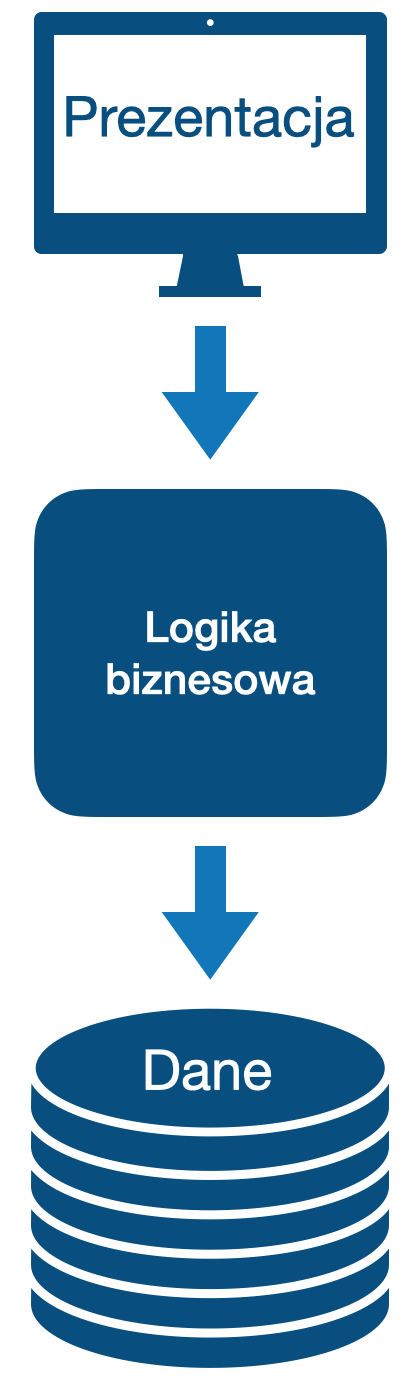
\includegraphics[scale=0.30]{patterns/three-layer.png}
    \end{center}

    \subsection{Model View Controller}

    Wzorzec architektoniczny, dzielący system na trzy główne części:
    \begin{enumerate}
        \item \textbf{Model}

        Reprezentuje podstawową część funkcjonalności systemu

        \item \textbf{Widok}

        Wyświetla dane dostarczone przez model użytkownikowi

        \item \textbf{Kontroler}

        Przyjmuje dane wejściowe od użytkownika oraz przetwarza jego żądania

    \end{enumerate}

    \begin{center}
        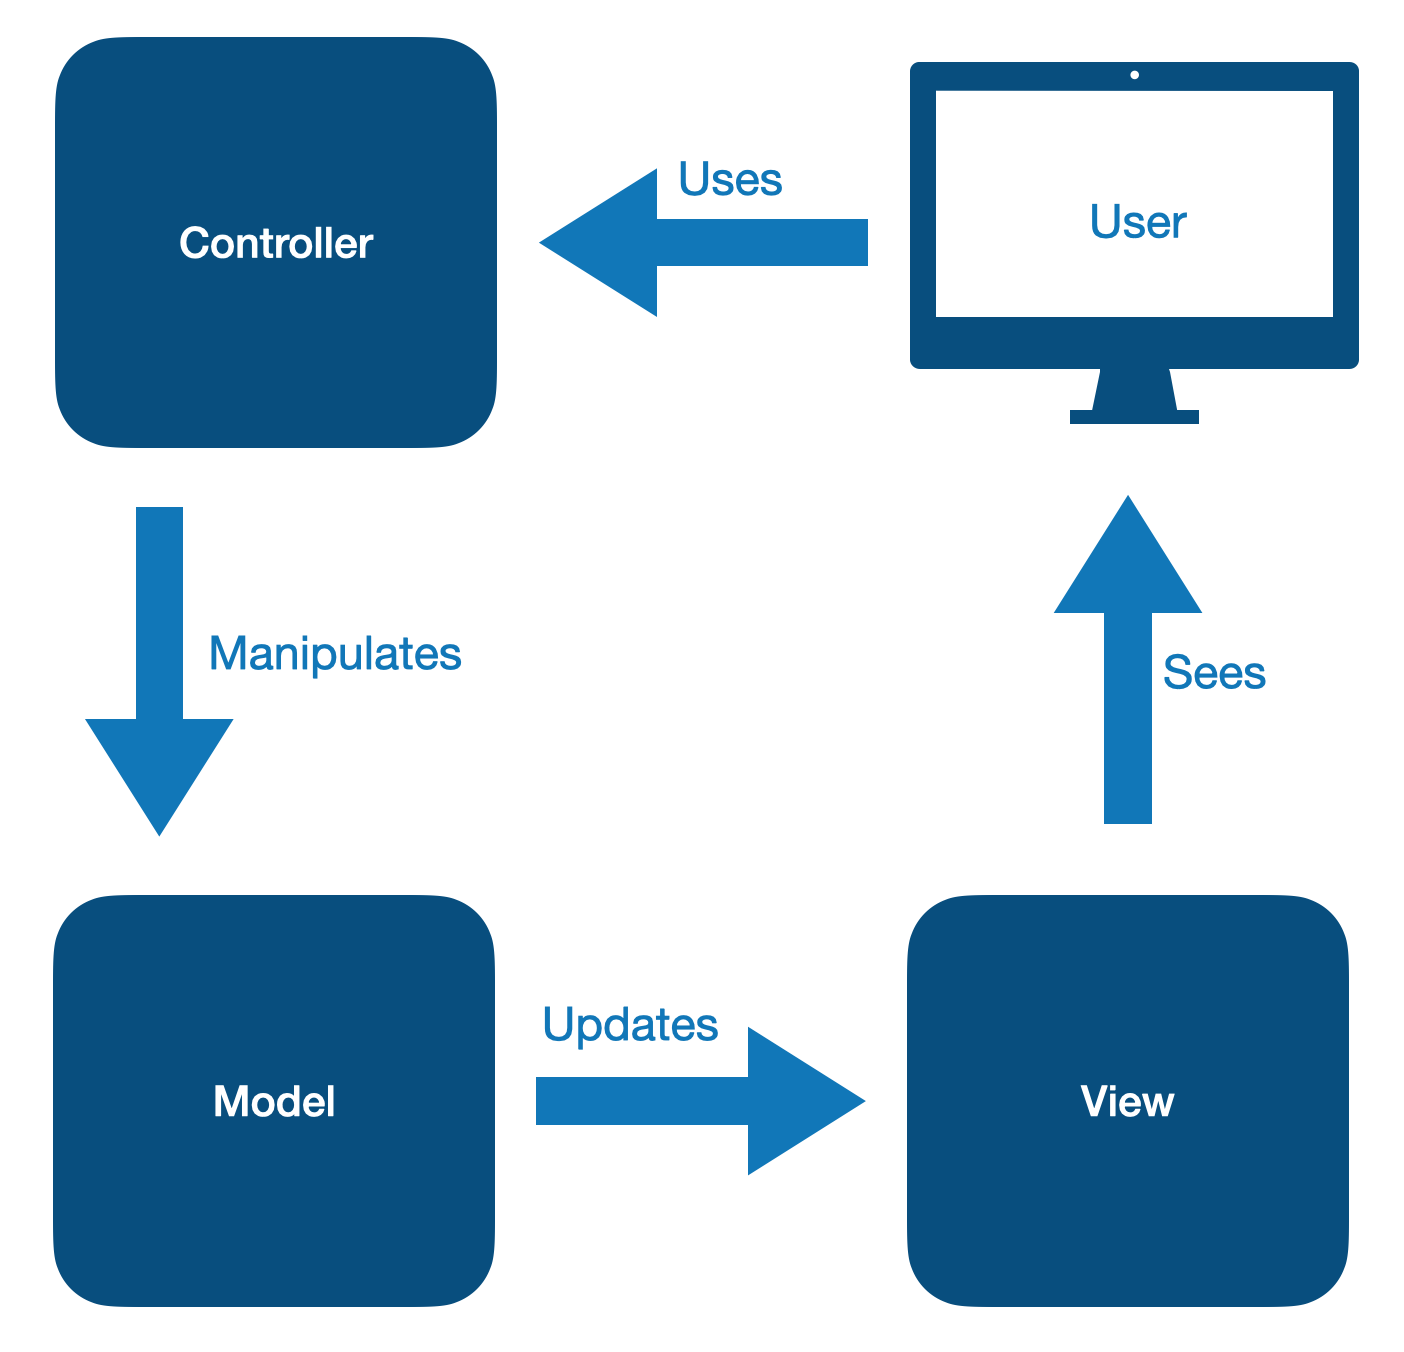
\includegraphics[scale=0.30]{patterns/mvc.png}
    \end{center}

    Przykłady:
    \begin{itemize}
        \item Smalltalk
        \item Swing
    \end{itemize}

    \subsection{Pipeline (filtry i potoki)}

    Wzorzec Pipeline pozwala na uporządkowanie systemu, która przetwarza
    strumienie danych. Każdy krok przetwarzania jest zamknięty w filtrze
    Dane przesyłane są pomiędzy elementami za pomocą potoków (pipes).

    \begin{center}
        \includegraphics[scale=0.30]{patterns/pipeline.png}
    \end{center}

    Przykłady:
    \begin{itemize}
        \item Unix pipeline
        \item Multimedia (GStreamer, Membrane)
    \end{itemize}

    \subsection{Client - Server}

    Architektura ta polega na podziale systemu na dostawcę usług (server)
    oraz ich odbiorców (clients). Serwer oczekuje na żądania (request) klientów,
    przetwarza je, a następnie wysyła odpowiedzi (response). Pracuje zatem, w
    przeciwieństwie do klientów, w trybie pasywnym.

    \begin{center}
        \includegraphics[scale=0.30]{patterns/client-server.png}
    \end{center}

    Przykłady:
    \begin{itemize}
        \item Serwer WWW i przeglądarka internetowa
        \item System bankowy
    \end{itemize}

    \newpage
    \subsection{Peer-to-Peer}

    Każdy z podsytemów (hostów, peerów) może pełnić zarówno funkcję
    serwera, jak i klienta. Architektura systemu jest rozproszona, każdy
    z hostów ma te same uprawnienia.

    \begin{center}
        \includegraphics[scale=0.30]{patterns/peer2peer.png}
    \end{center}

    Przykłady:
    \begin{itemize}
        \item Torrenty
        \item Videochaty (nie zawsze)
    \end{itemize}

    \newpage

\end{document}
